\documentclass{beamer}
% \usepackage[utf8]{inputenc}
\usetheme{Madrid}
\usecolortheme{beaver}
\usepackage{booktabs}
\usepackage{siunitx}
\usepackage{diagbox}
\usepackage{amsmath}
\usepackage{hyperref}
\usepackage{graphicx}
\usepackage{xeCJK}
\usepackage[
backend=biber,
style=apa,
]{biblatex}
\usepackage[export]{adjustbox}
\usepackage{booktabs}
\usepackage{siunitx}
\newcolumntype{d}{S[
    input-open-uncertainty=,
    input-close-uncertainty=,
    parse-numbers = false,
    table-align-text-pre=false,
    table-align-text-post=false
 ]}
\addbibresource{references.bib}
%------------------------------------------------------------
%This block of code defines the information to appear in the
%Title page
\title[Spark 社科量化系列课程 10] %optional
{研究规范和道德}
\subtitle{Research Protocol and Ethics}

\author[杨点溢] % (optional)
{杨点溢}

\institute[LSE] % (optional)
{
  Department of Government\\
  London School of Economics and Political Science
}

\date[10 Sept 2023] % (optional)
{Spark 社科量化系列课程}

\logo{
\includegraphics[height=1cm]{spark.jpg}}

%End of title page configuration block
%------------------------------------------------------------



%------------------------------------------------------------
%The next block of commands puts the table of contents at the 
%beginning of each section and highlights the current section:

\AtBeginSection[]
{
  \begin{frame}
    \frametitle{本节课内容}
    \tableofcontents[currentsection]
  \end{frame}
}
%------------------------------------------------------------
\begin{document}

%The next statement creates the title page.
\frame{\titlepage}


%---------------------------------------------------------
%%This block of code is for the table of %contents after
%the title page
%\begin{frame}
%\frametitle{Table of Contents}
%\tableofcontents
%\end{frame}
%---------------------------------------------------------
\section{Null Results}
\begin{frame}{Null Results 空结果/零结果}
\begin{itemize}
    \item 当我们说"null results"的时候，指的是在\alert{统计功效}(statistical power)足够强时，仍然不能够拒绝零假说(null hypothesis)的结果。
    \item \textbf{统计功效 statistical power}:是指在对于影响大小和样本差别分布(sampling variability)的假设正确的情况下，研究显著的几率
\end{itemize}
\end{frame}

\begin{frame}{}
\begin{figure}
    \centering
    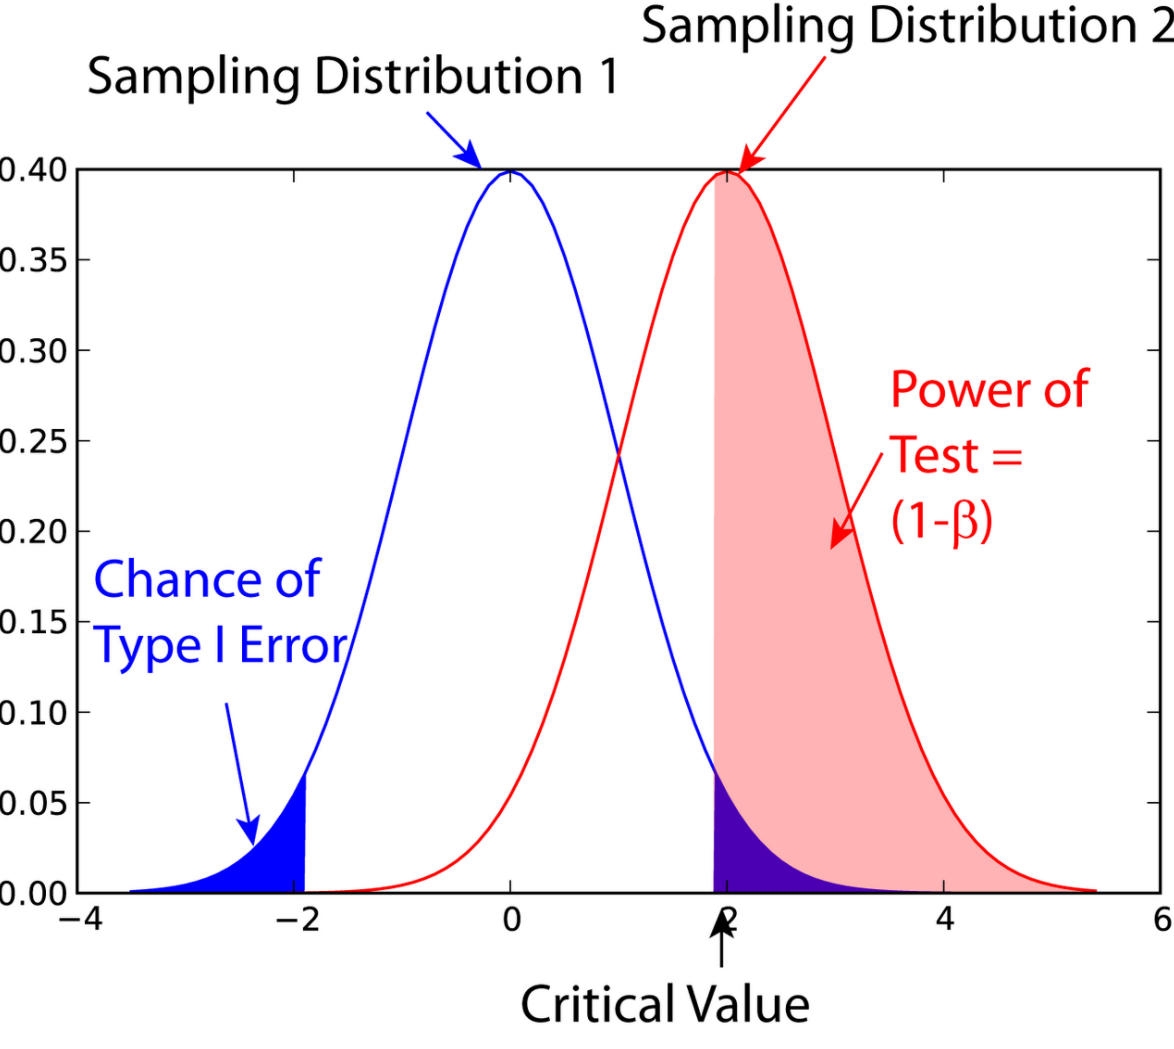
\includegraphics[width=0.6\linewidth]{power.png}
\end{figure}
\begin{itemize}
    \item $\alpha=$Chance of Type I error假阳$=$significance level显著等级
    \item $\beta=$Chance of Type II error假阴; $1-\beta=$统计功效 statistical power
\end{itemize}
\end{frame}

\begin{frame}{统计功效 Statistical power}
\begin{itemize}
    \item 当我们思考统计功效时，我们需要问自己：最小的可以被探测到的影响大小(minimal detectable effect or MDE)是多少？多大的影响算是“有意义”呢？
    \item 这有时候取决于前人的研究，但是思考一下“抽屉问题” (file drawer proble).
    \item 今天，绝大多数统计功效研究(power analysis)是基于模拟(simulation-based)的，应该能够完全一致地模拟你的研究(比如说样本大小）下面是一些功效模拟的工具网站：
    \begin{itemize}
        \item \href{https://aaroncaldwell.us/SuperpowerBook/}{Superpower}
        \item \href{https://declaredesign.org/}{DeclareDesign}
        \item \href{https://egap.shinyapps.io/power-app/}{EGAP shiny app (for experiments)}
    \end{itemize}
\end{itemize}
\end{frame}

\begin{frame}{"Underpowered" nulls 低效零结果}
\begin{itemize}
    \item 指的是我们不能够拒绝零假说，但是样本差异太大或者/且我们的样本量($N$)太小.
    \item 这时有可能我们测量到了一个很大的影响，但是还是不能拒绝零假说（不显著）
    \item 低效零结果(underpowered nulls)提供不了什么信息
    \begin{itemize}
        \item 研究\alert{设计}就有问题
    \end{itemize}
    \item 能不能出显著结果全看脸
\end{itemize}
\end{frame}

\section{可信度危机 Credibility Crisis}
\begin{frame}{“不显著”(Null results)带来的问题}
由于“不显著”的结果难以排除Type II Error(功效不够带来的假阴)，而且往往“没那么有意思”（没有发现影响），往往在投稿时低人一等。
\begin{itemize}
    \item 以前问题比较大，现在好一点，但仍然属于“政治正确”
\end{itemize}
这会造成\alert{可信度危机 credibility crisis}（整个学科的偏差）：
\begin{enumerate}
    \item <2->学术不端/造假 Misconduct/fraud
    \begin{itemize}
        \item 理论上来讲还是比较好解决的（只要编辑部看的话，如果不看另说）
    \end{itemize}
    \item <3->P-hacking(screening)/multi-hypotheses testing/researcher degrees of freedom
    \begin{itemize}
        \item P-hacking/screening:排列组合，哪个显著了展示哪个，然后编故事
        \item Researcher degrees of freedom 研究者自由度：研究设计的微妙选择（外行看不出来）
    \end{itemize}
    \item <4->复现危机 Replication Crisis
    \begin{itemize}
        \item 别人复现不出来（心理学、经济学、政治科学、医学...）
    \end{itemize}
    \item <5->出版偏差 Publication bias
    \begin{itemize}
        \item 只有一部分结果（通常是显著的）才得以发表
    \end{itemize}
\end{enumerate}
\end{frame}

\begin{frame}{证据 /1 (\cite{van_zwet_2021})}
\begin{figure}
    \centering
    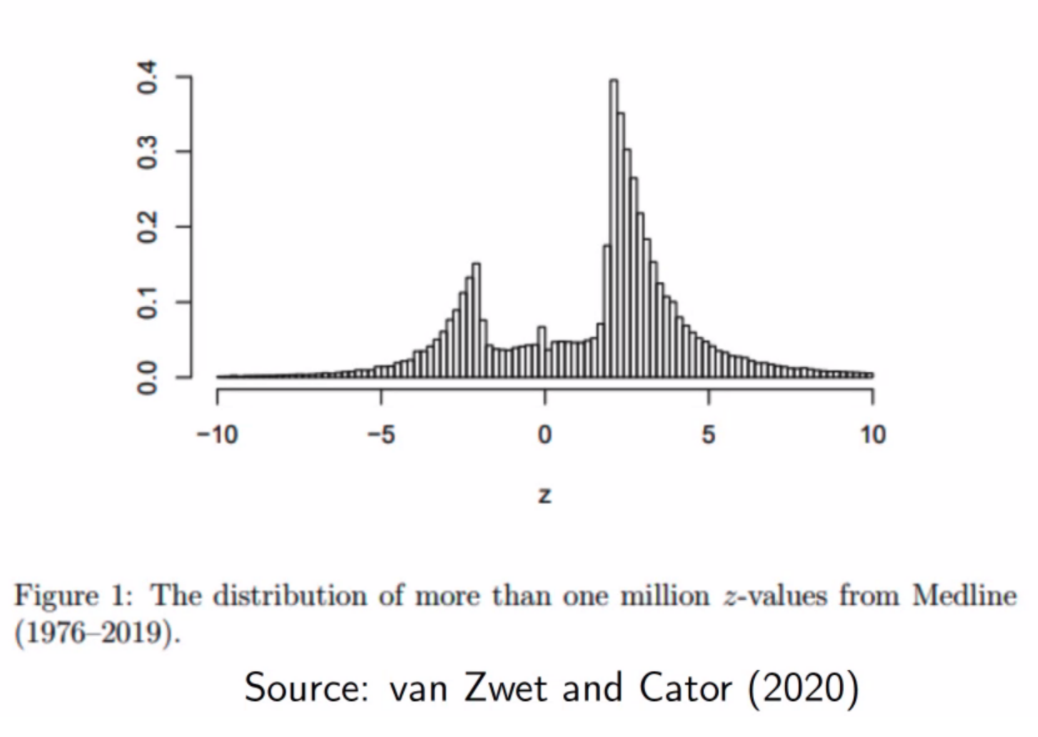
\includegraphics[width=0.8\linewidth]{evidence.png}
\end{figure}
\end{frame}

\begin{frame}{证据 /2 (from Twitter)}
研究被毙 Killed projects!
\begin{figure}
    \centering
    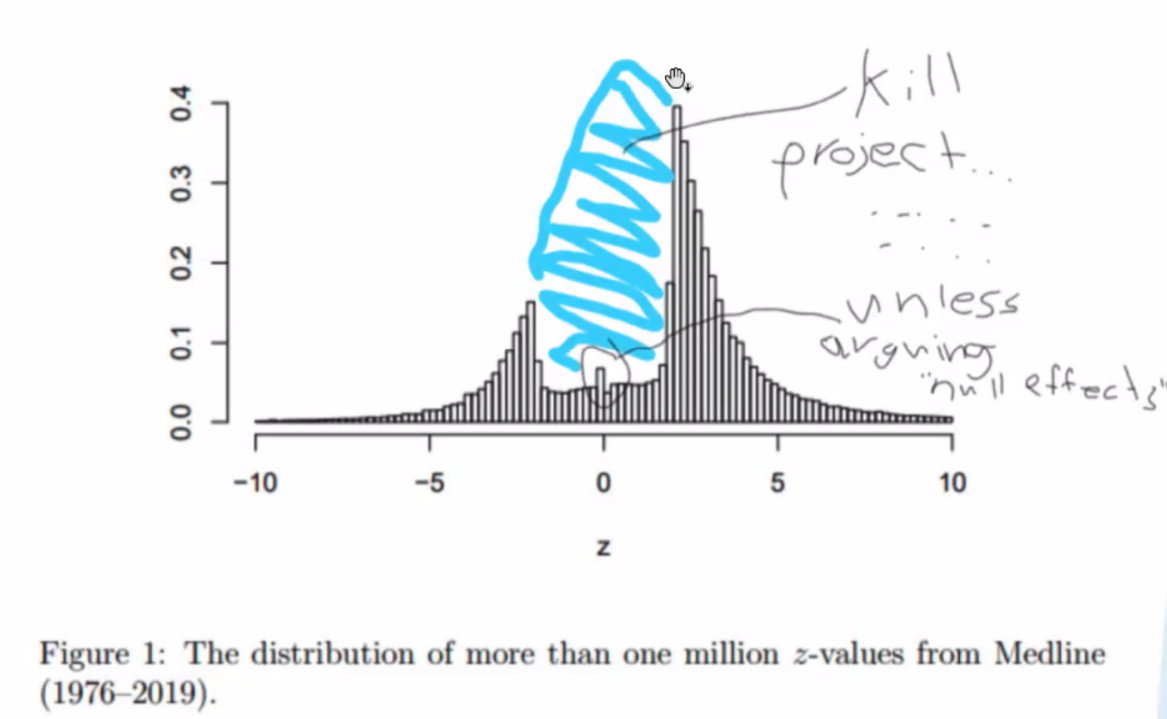
\includegraphics[width=0.8\linewidth]{evidence2.png}
\end{figure}
往好了想：可能只是知难而退，或者有把握了才做研究。
\end{frame}

\begin{frame}{可信度危机的深层原因是什么？}
\begin{figure}
    \centering
    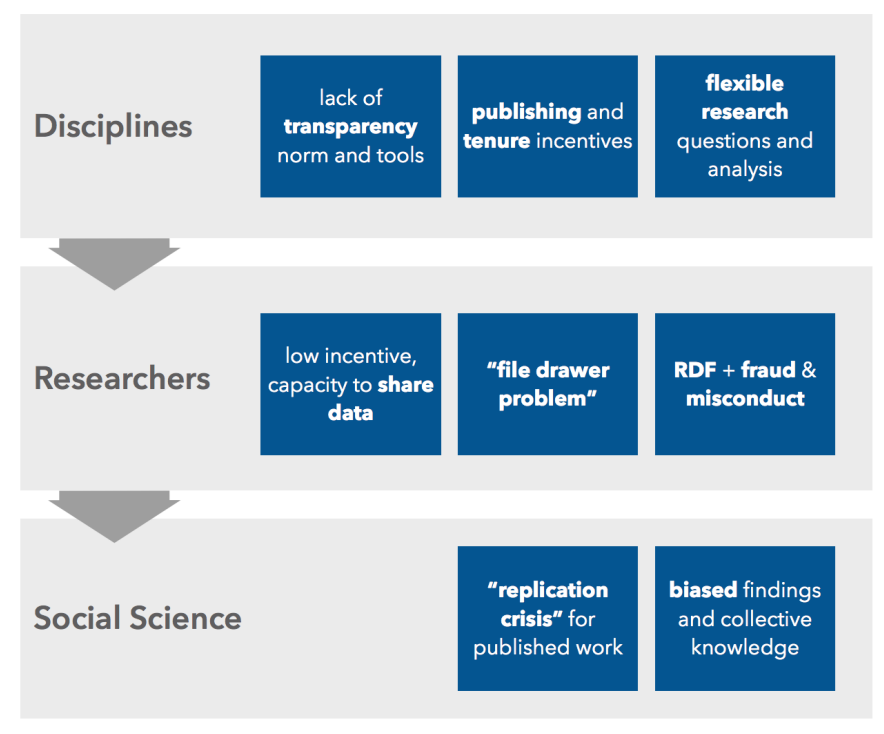
\includegraphics[width=0.7\linewidth]{crisis.png}
\end{figure}
\end{frame}

\begin{frame}{出版偏差（aka 抽屉问题 file drawer problem）}
\begin{itemize}
    \item \textbf{问题}：显著的研究更有可能被提交/发表$\Rightarrow$我们看不见零结果/阴性结果的研究
    \item \textbf{结果}：学术界系统性偏差：发表的文章可能只是“随机”地显著(比如说5\%的显著性水平意味着5\%的实际没有的影响也会显著)
\end{itemize}
\end{frame}

\begin{frame}{另一些证据 /3 (\cite{Fanelli2012})}
不同科学学科显著结果的比例
\begin{figure}
    \centering
    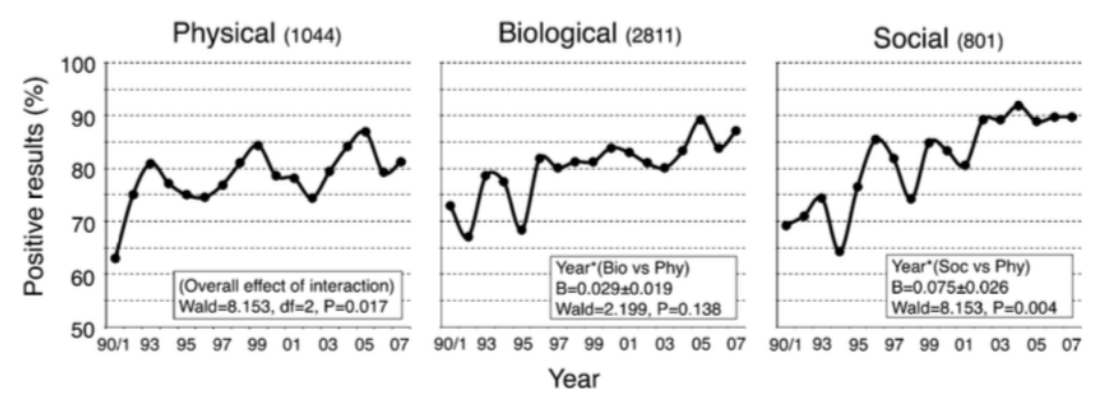
\includegraphics[width=0.9\linewidth]{evidence3.png}
\end{figure}
\end{frame}

\begin{frame}{另一些证据 /4 (\cite{Franco2014})}
(社会科学)强结果被写出来的可能性比零结果高60pp；发表的可能性高40pp
\begin{figure}
    \centering
    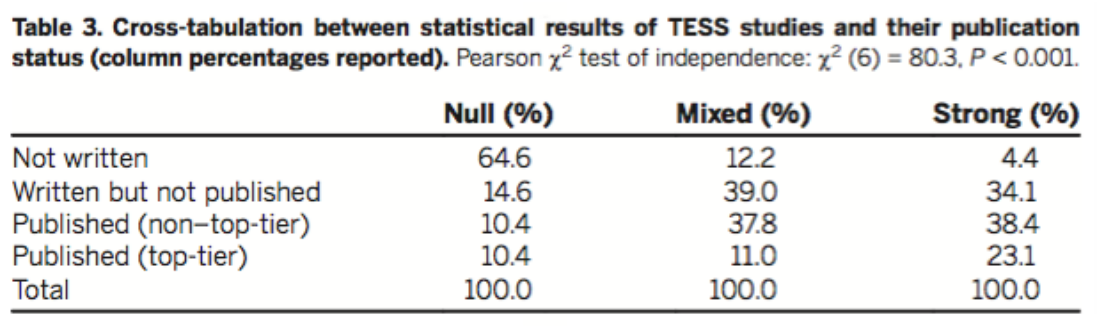
\includegraphics[width=0.9\linewidth]{evidence4.png}
\end{figure}
\end{frame}

\begin{frame}{P-hacking}
"If you torture the data long enough, it will confess." - Ronald Coase
\begin{itemize}
    \item \textbf{机会}：研究者可能在研究设计和分析方面有很多“自由度”$\rightarrow$p-hacking (但不一定是可以的！详见 \cite{Gelman2019TheGO})
    \item \textbf{动机}：研究者有动机追求显著结果（期刊、教职、退休压力等）
    \item \textbf{结果}：有偏差的实证证据（同时也导致复现危机）
\end{itemize}
\end{frame}

\begin{frame}{案例：鲨鱼袭人和投票 (\cite{AchenBartels})}
\begin{figure}
    \centering
    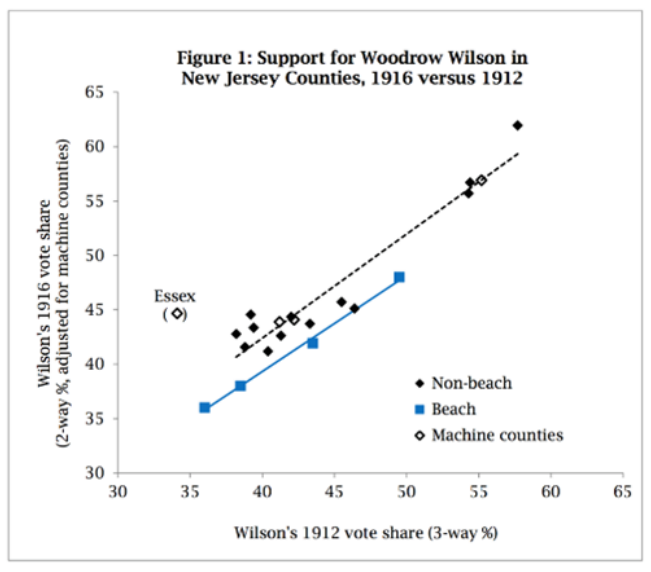
\includegraphics[width=0.6\linewidth]{shark.png}
\end{figure}
"A dramatic series of shark attacks in NJ in 1916... voters significantly
punished the incumbent president at the polls"
\end{frame}

\begin{frame}{对Achen \& Bartels (\citeyear{AchenBartels})的反驳 (\cite{Fowler2018})}
\begin{itemize}
    \item \alert{相关性}：不同县域的选举结果不是独立的（实际意义上的“样本量”可能受限）
    \item \alert{不同路径 forking paths}: 分析同样的数据可能有不同的路径（e.g.如何处理“异常值”outliers）
\end{itemize}
~\\
'We assemble data on every fatal shark attack in U.S. history and
county-level returns from every presidential election between 1872 and
2012, and we find little systematic evidence that shark attacks hurt
incumbent presidents or their party.'
\end{frame}

\section{复现 Replication}
\begin{frame}{复现 Replication}
\begin{itemize}
    \item 复现可以意味着不同的事情：
    \begin{enumerate}
        \item 所有的图表结果都可以使用相同的数据（和代码）的情况下得到一样的结果。
        \item 同样的研究设计在\alert{类似}的情景下可以得到相似的结果
        \item 同样的研究可以在\alert{不同}的情境下得到相似的结果
    \end{enumerate}
    \item 但是社会、行为和医学科学的研究往往不能复现 （复现危机）
    \begin{itemize}
        \item 理论上，复现可以测试原结果是\alert{稳健的} robust 还是仅仅是\alert{随机 random}的结果
        \item 现实中，复现的失败可能是以下的结果
        \begin{itemize}
            \item 数据/代码分享的不透明
            \item 数据/代码的小错误errors
            \item 学术造假/不端
        \end{itemize}
    \end{itemize}
\end{itemize}
\end{frame}

\begin{frame}{潮流：数据和代码开放}
\begin{itemize}
    \item 解决最低级别的复现危机$\Rightarrow$开源
    \item 随着时代的进步，越来越多的期刊要求作者在指定数据源(dataverse)公开数据及代码 （否则不予发表）
    \begin{itemize}
        \item 比较流行的：哈佛大学 Harvard Dataverse
        \item 国内这方面差一点
    \end{itemize}
    \item 一些期刊会聘请复现编辑(replication editors)或者数据编辑(data editors)来复现结果，只有复现成功才能发表
    \begin{itemize}
        \item 但是顶刊AJPS都很拉
    \end{itemize}
\end{itemize}
\end{frame}

\begin{frame}{论编辑的不仔细 文章来源：\cite{Shoub2021}}
    \begin{figure}
    \centering
    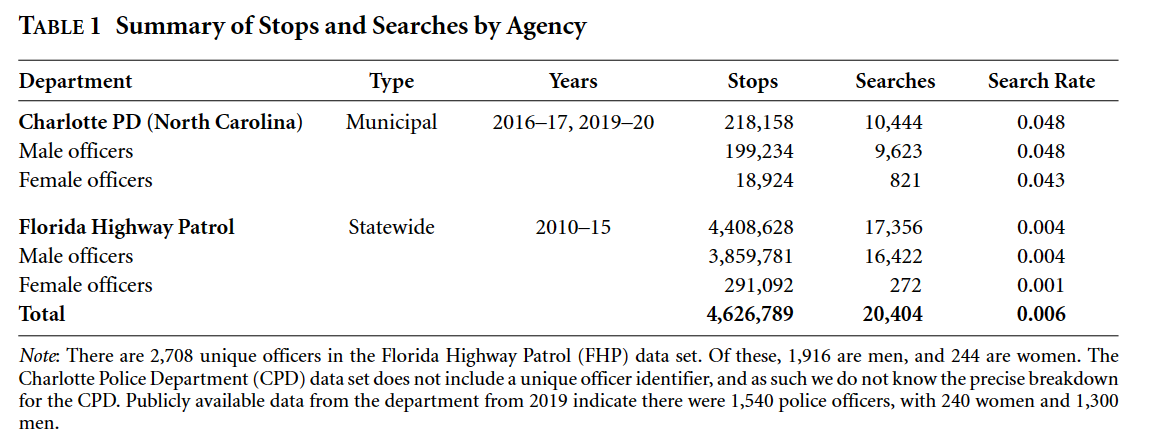
\includegraphics[width=0.9\linewidth]{femaleoff.png}
    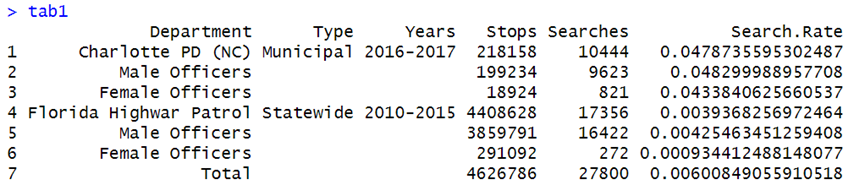
\includegraphics[width=0.9\linewidth]{femaleoff_rep.png}
\end{figure}
\end{frame}

\begin{frame}{案例：被撤稿的金融顶刊文章 (\cite{Rampini2020})}
\begin{figure}
    \centering
    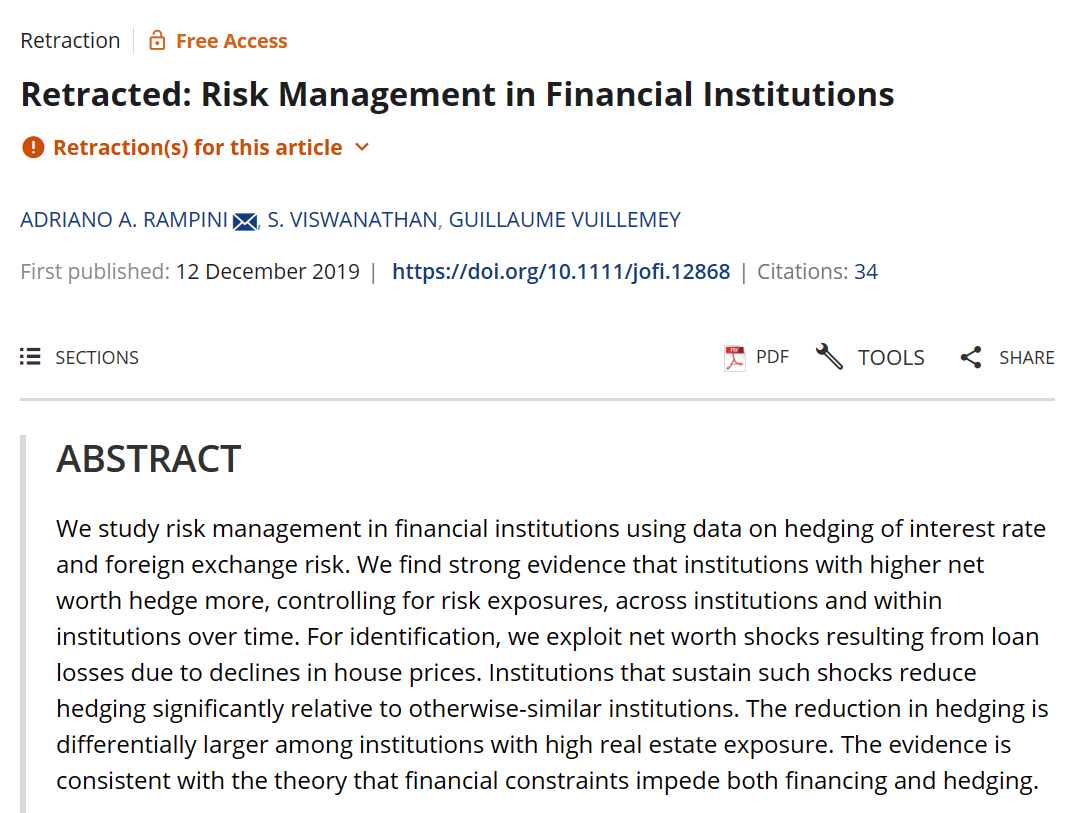
\includegraphics[width=0.8\linewidth]{retracted.png}
\end{figure}
\end{frame}

\begin{frame}{朴实无华的造假 /1 (\cite{Guest2021})}
    \begin{figure}
    \centering
    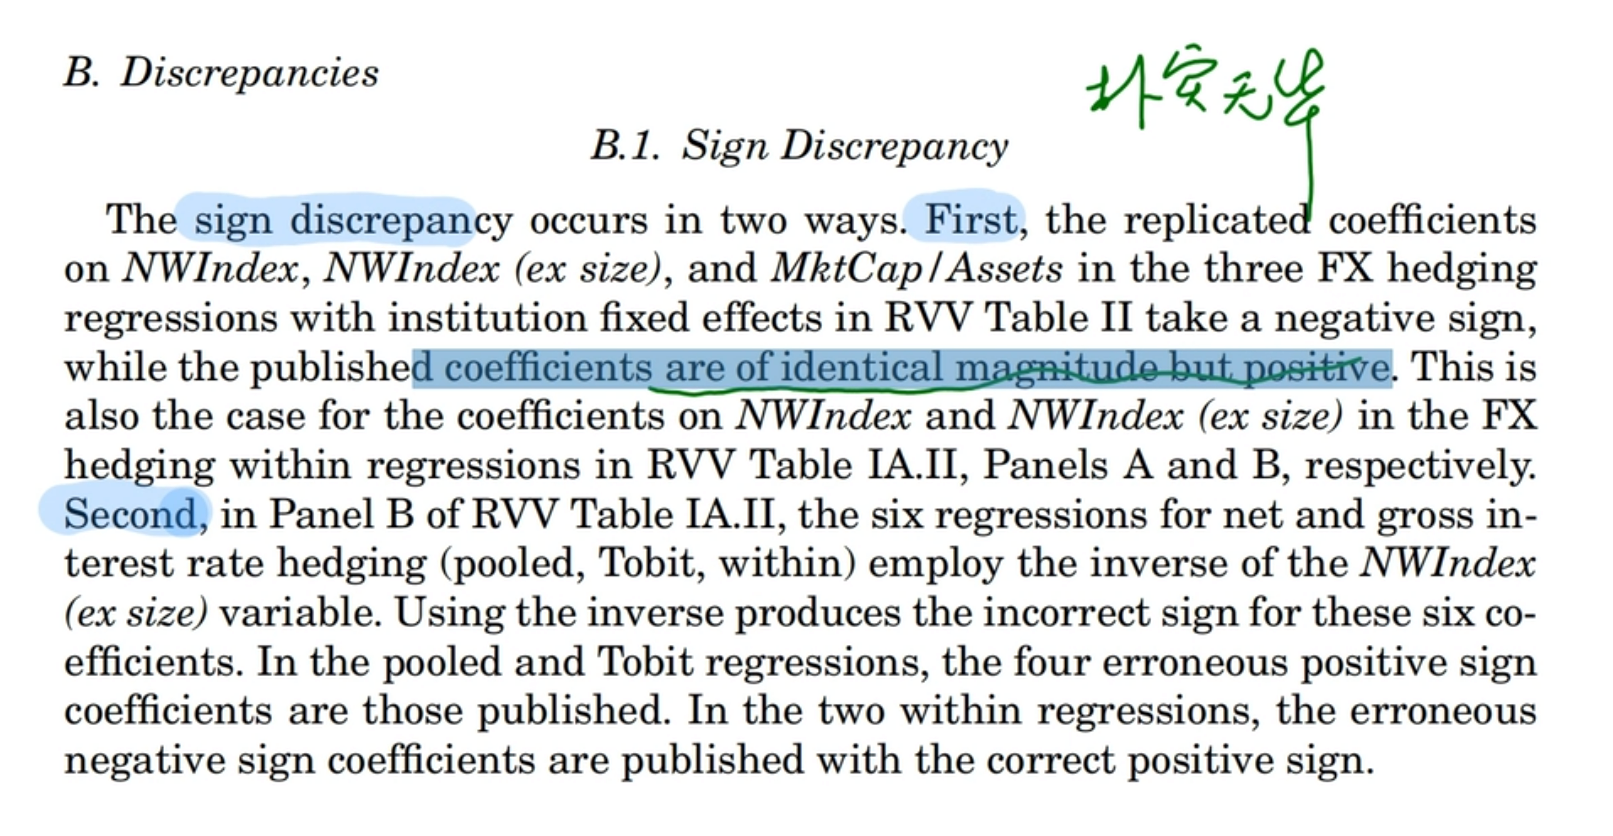
\includegraphics[width=0.8\linewidth]{changesign.png}
\end{figure}
B站链接:\url{https://www.bilibili.com/video/BV1rg4y177zC/}
\end{frame}

\begin{frame}{朴实无华的造假 /2 (\cite{Guest2021})}
    \begin{figure}
    \centering
    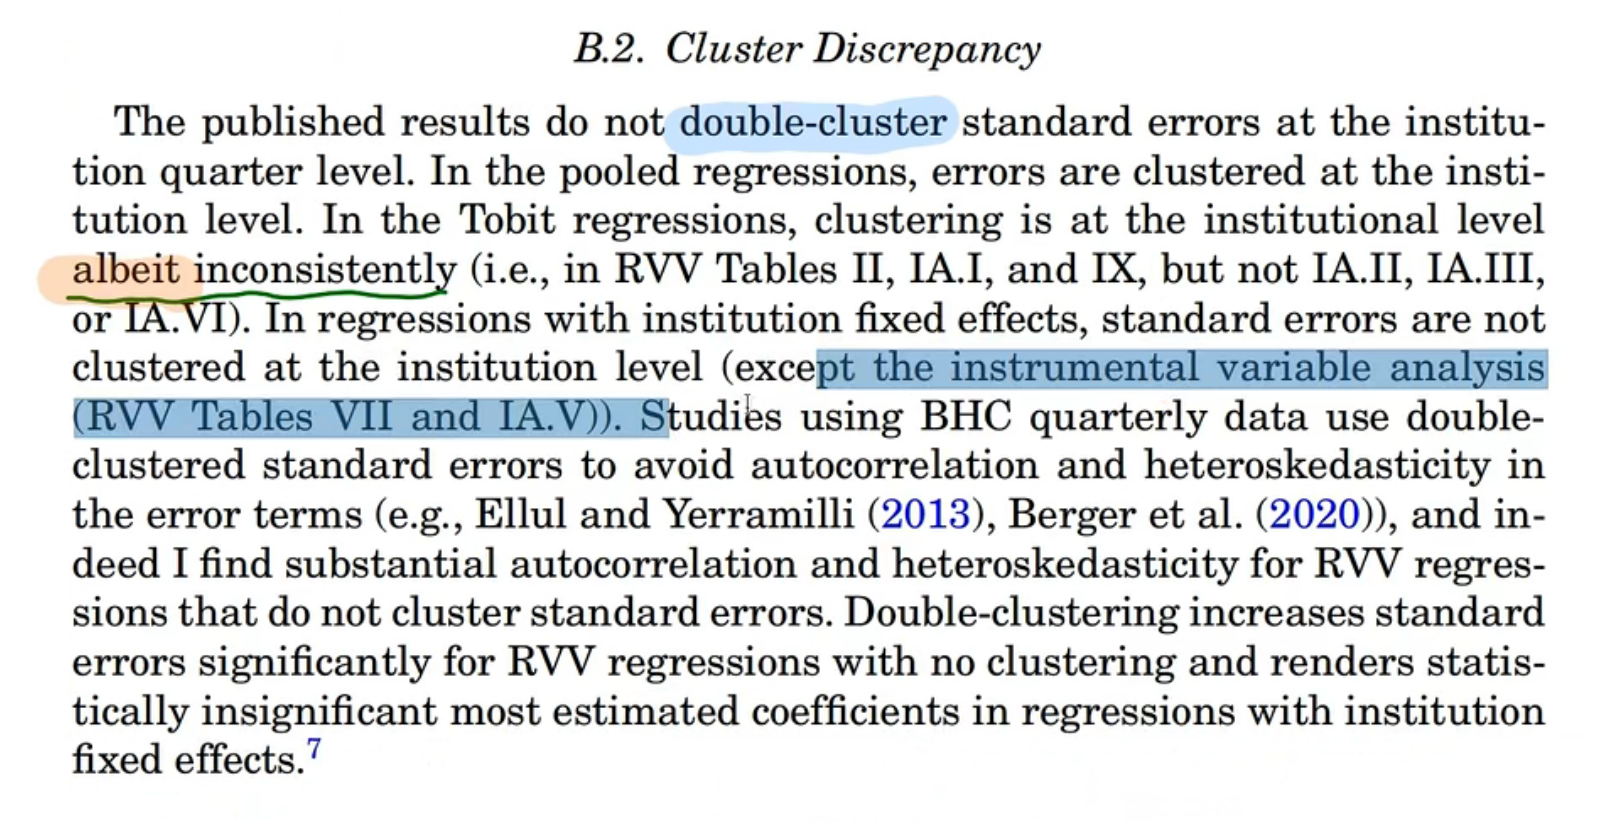
\includegraphics[width=0.8\linewidth]{wrongcluster.png}
\end{figure}
B站链接:\url{https://www.bilibili.com/video/BV1rg4y177zC/}
\end{frame}

\section{可信度危机的解决办法}
\begin{frame}{可信度危机（包括复现危机）有什么解决办法？}
\begin{itemize}
    \item 学术界整体的习惯也在变化
    \item 新的工具和标准正在逐步影响\alert{整个研究生命周期} research lifecycle.
    \begin{itemize}
        \item Berkeley Initiative for Transparency in Social Sciences (\href{https://www.bitss.org/}{BITSS})
        \item Open Science Framework (\href{https://osf.io/}{OSF})
        \item \href{https://dataverse.org/}{Dataverse}
        \item Evidence in Governance and Politics (\href{https://egap.org/}{EGAP})
        \item Institute for Replication (\href{https://i4replication.org/}{I4R})
    \end{itemize}
\end{itemize}
\end{frame}

\begin{frame}{研究生命周期：个人级别解决方案}
    \begin{figure}
    \centering
    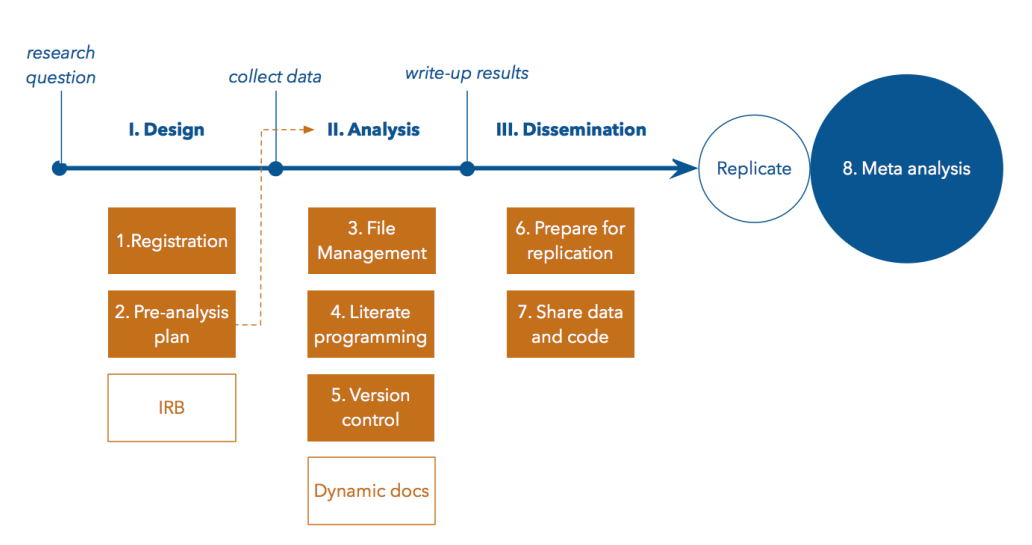
\includegraphics[width=0.9\linewidth]{individual_solution.png}
\end{figure}
\end{frame}

\begin{frame}{研究设计阶段 Research Design}
\begin{figure}
    \centering
    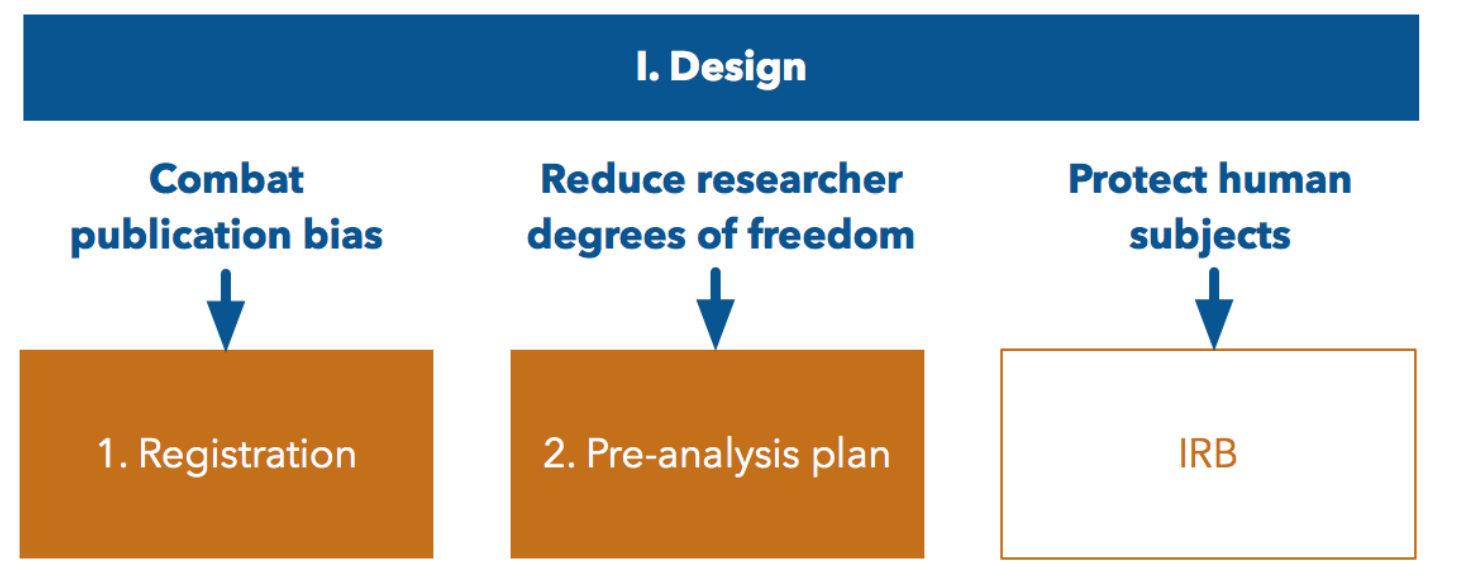
\includegraphics[width=0.9\linewidth]{design.png}
\end{figure}
\end{frame}

\section{研究前的登记与预分析计划}
\begin{frame}{Registration 登记}
\begin{itemize}
    \item 在开始研究前就要在指定\alert{注册表 registry}“登记”
    \begin{itemize}
        \item 2021年1月1日起所有在\textit{Journal of Politics}投稿的实验类研究都要预先登记
    \end{itemize}
    \item \textbf{原因}：为了避免抽屉问题(file drawer problem)和出版偏差(publication bias)
    \item 在哪登记呢？
    \begin{itemize}
        \item \href{https://osf.io/}{Open Science Framework}
        \item \href{https://www.socialscienceregistry.org/}{American Economics Association (AEA)} (别误会，对所有社会科学开放)
        \item \href{https://aspredicted.org/}{As Predicted (Wharton)}
    \end{itemize}
    \item 登记什么内容呢？马上讲
\end{itemize}
\end{frame}

\begin{frame}{预分析计划 Pre-Analysis Plans (PAPs)}
\begin{itemize}
    \item PAP是对于\alert{研究设计}和\alert{数据分析}的详细描述，于\alert{得到数据前}提交给注册表registry.
    \begin{itemize}
        \item 简单规则：PAP应该详细到一个这个细分领域的专家拿到你的PAP之后复刻得到一样的结果（如果拿到数据）
    \end{itemize}
    \item 原因：
    \begin{enumerate}
        \item “把手绑住” tie your hands （限制研究者自由度）
        \item 区分\textit{验证性(confirmatory)}和\textit{探索性exploratory}分析
        \item 为研究的可信度背书
        \item 方法的公开有助于别人基于你的基础上进一步研究
    \end{enumerate}
\end{itemize}
研究前的登记往往（至少）包括一个预分析计划(PAP).
\begin{itemize}
    \item \textbf{登记一定程度上解决了出版偏差}：无论怎样研究都“存在”在数据库里了
    \item \textbf{PAP同时防止了P-hacking}: 限制研究者自由度
\end{itemize}
\end{frame}

\begin{frame}{预分析计划}
并不是唯一的标准，但往往包括...
\begin{figure}
    \centering
    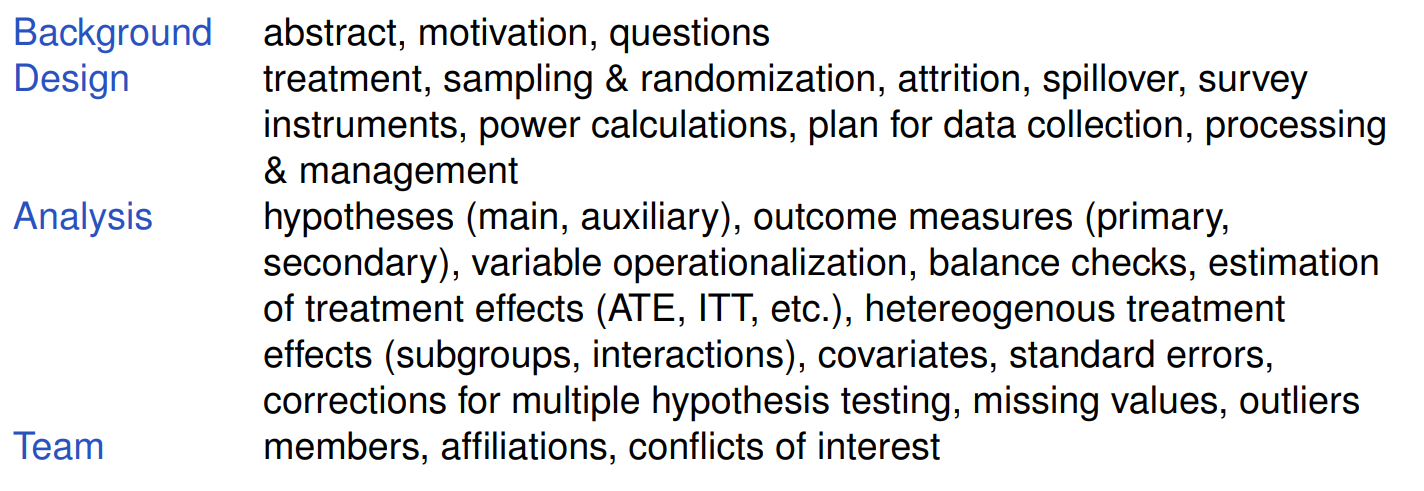
\includegraphics[width=\linewidth]{pap.png}
\end{figure}
\end{frame}

\begin{frame}{Olken's PAP Checklist (\cite{Olken2015})}
    \begin{figure}
    \centering
    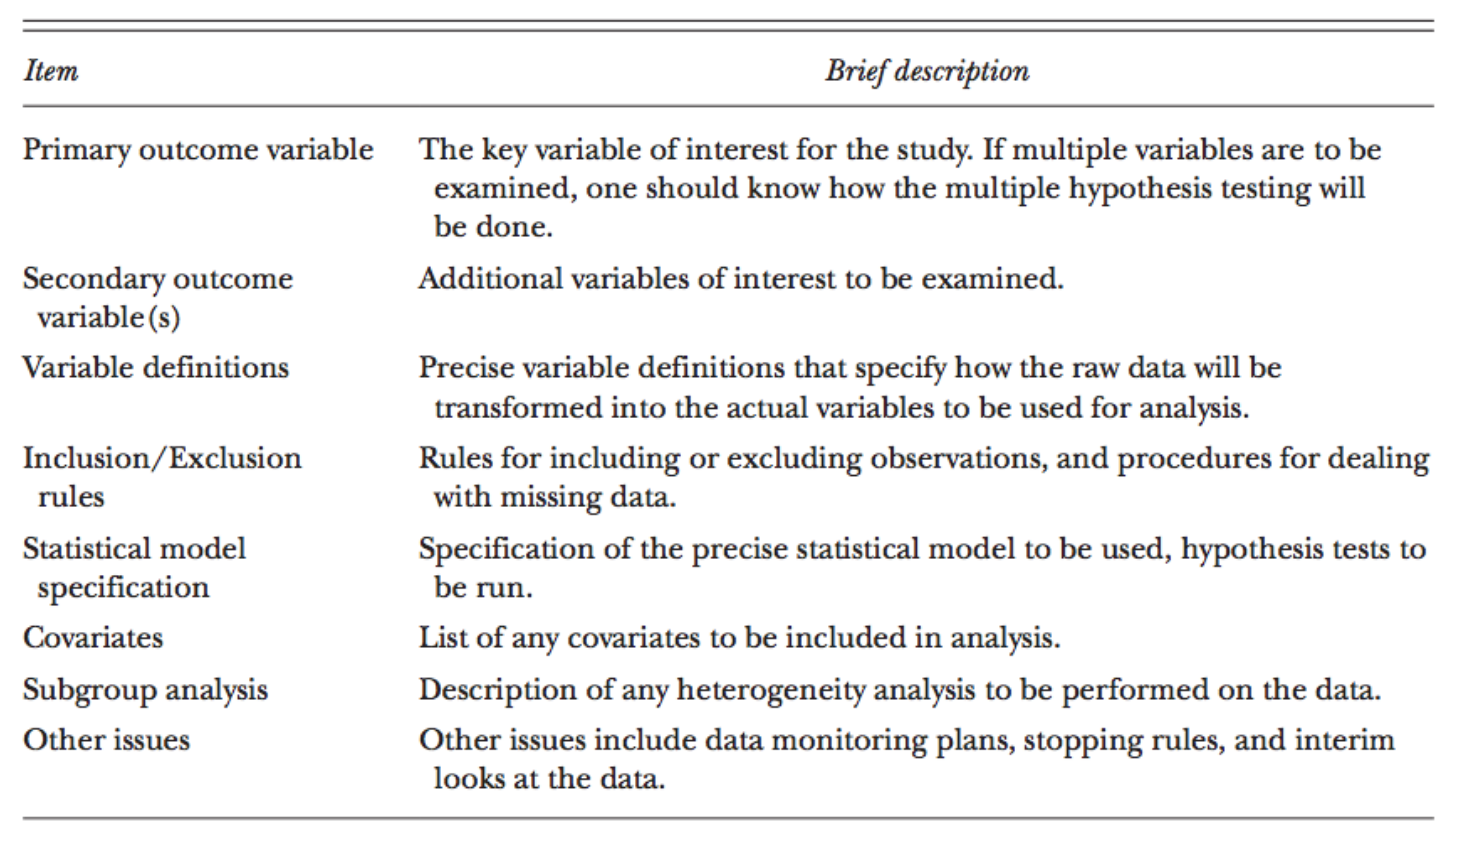
\includegraphics[width=0.9\linewidth]{papchecklist.png}
\end{figure}
\end{frame}

\begin{frame}{但是有一些取舍...}
会不会在研究的过程中发现了纰漏？会不会研究中“灵机一动”有了不得的发现？会不会同时有机会探索其它问题？
    \begin{figure}
    \centering
    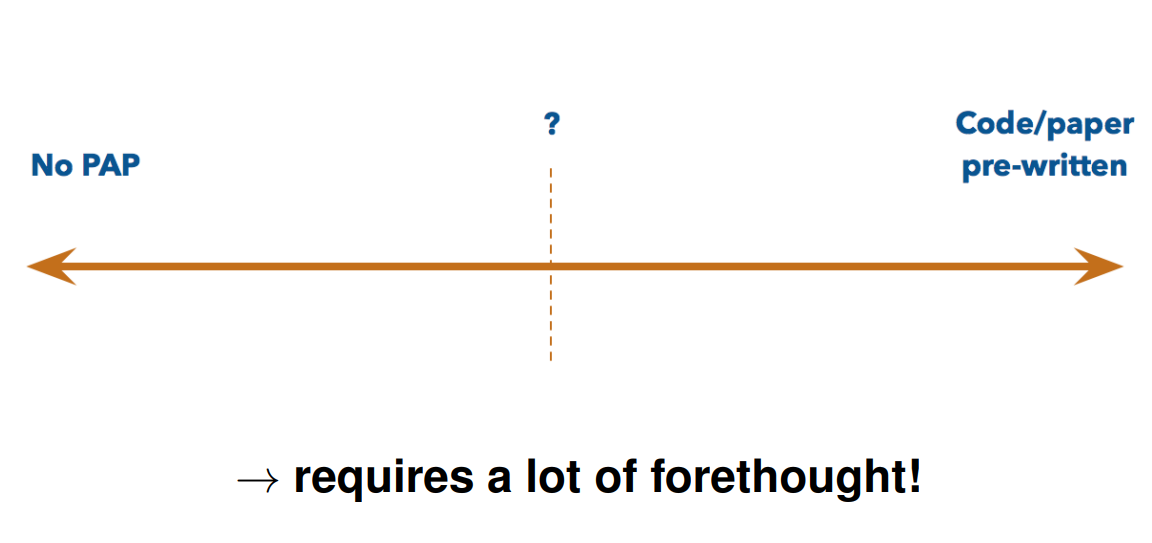
\includegraphics[width=0.9\linewidth]{tradeoff.png}
\end{figure}  
\end{frame}

\begin{frame}{坐标轴最右端: Registered Reports}
\begin{itemize}
    \item Registered Reports是最极端的登记形式：作者在研究开始\alert{之前}就向期刊提交了文章
    \item 这个“还没开始单已经写好了”的文章包括了所有的分析和表格，仅仅是没有数据
    \item 有些期刊已经尝试了，并且至少有一个主要刊物(\textit{Journal of Politics})正在考虑引进这一制度。
\end{itemize}
问题？
\begin{itemize}
    \item 量化帝国主义？
    \item 加剧已有的权力不平衡？
\end{itemize}
\end{frame}

\section{IRB:对于人类对象的保护}

\begin{frame}{Institutional Review Board (IRB)/道德审核过程}
\begin{itemize}
    \item 如果你的研究涉及在人类对象进行实验收集（实验、采访、问卷...），你需要通过道德审查
    \begin{itemize}
        \item 你的机构的道德审查委员会(Institutional Review Board)会负责
    \end{itemize}
    \item 通过道德审查\alert{不意味着}你的研究是道德的，只是没踩红线而已
    \item IRB的严格程度在每个国家和每个机构都是不一样的
    \item IRB会要求你对研究过程做出修改/要求你对实验过程/提问问题有更详细的介绍
    \item 可能会有听证会
\end{itemize}
\end{frame}

\begin{frame}{The Belmont Report /1}
\begin{itemize}
    \item The Belmont report (\citeyear{Belmont1979})是第一个提出涉及人类对象研究伦理准则的文件。
    \item 是对早前医生和研究者对人权侵犯的回应
    \begin{itemize}
        \item 纳粹德国  (纽伦堡审判)
        \item 美国 （梅毒实验 syphilis experiment）和 斯坦福监狱实验
        \item （没提的）日本
    \end{itemize}
\end{itemize}
\end{frame}

\begin{frame}{The Belmont Report /2}
准则：
\begin{itemize}
    \item 对人的尊重 Respect for Persons
    \item 善意 Beneficence
    \item 正义 Justice
    \begin{itemize}
        \item $\approx$不见死不救not witholding life-saving support
    \end{itemize}
\end{itemize}
\end{frame}

\begin{frame}{美国政治科学协会(APSA) 伦理准则}
\begin{itemize}
    \item 在一年的辩论后于2020年批准
    \item 在\alert{实验}社群中非常有争议
    \item 被APSR（政治科学领域最重要的期刊）采纳
    \item 现在鼓励APSR评议员提出伦理质疑
\end{itemize}
\end{frame}

\begin{frame}{准则 Principles}
\begin{enumerate}
    \item 自主 Autonomy
    \item 个体研究者责任 Individual researcher responsibility
    \item 脱离需要解释 Deviations need justification
    \item 权力 power
    \item 同意 Consent
    \item 欺骗 Deception
    \item 伤害和创伤 Harm and trauma
    \item 保密性 Confidentiality
    \item 影响 Impact
    \item 法律和法规 Laws and regulations
    \item 责任 Responsibility
\end{enumerate}
\end{frame}

\begin{frame}{主要争论}
主要争论点为：
\begin{enumerate}
    \item 欺骗的使用/提供不完全的信息
    \item 缺少知情同意书informed consent
    \item 不平等权力关系 Unequal power relationships
    \item 对于政治、社会和民主结果的影响
\end{enumerate}
\end{frame}

\begin{frame}{知情同意书 Informed consent}
    \begin{itemize}
        \item 对象同意参与到一个研究中
        \item 对象完全知道作为研究参与者的权利以及如何对研究过程投诉
        \item 那么怎样不算有效的知情同意呢？
        \begin{itemize}
            \item 研究对象不理解知情同意书的内容
            \item 研究对象无法(unable)同意
        \end{itemize}
    \end{itemize}
\end{frame}

\begin{frame}{影响 Impact}
研究\alert{过程}产生的影响要纳入考量
    \begin{figure}
        \centering
        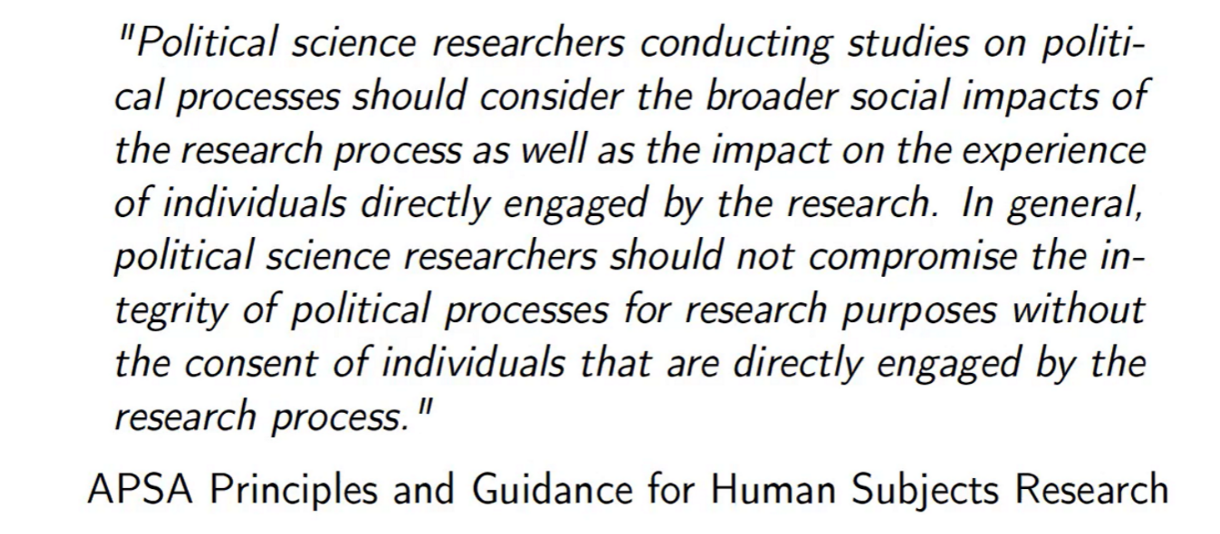
\includegraphics[width=\linewidth]{impact.png}
    \end{figure}
\end{frame}

\begin{frame}{合作伙伴 Partnerships}
\begin{itemize}
    \item 在由合作伙伴代为进行实验干涉(interventions)的情况下有一些道德考量的豁免
\end{itemize}
\begin{figure}
        \centering
        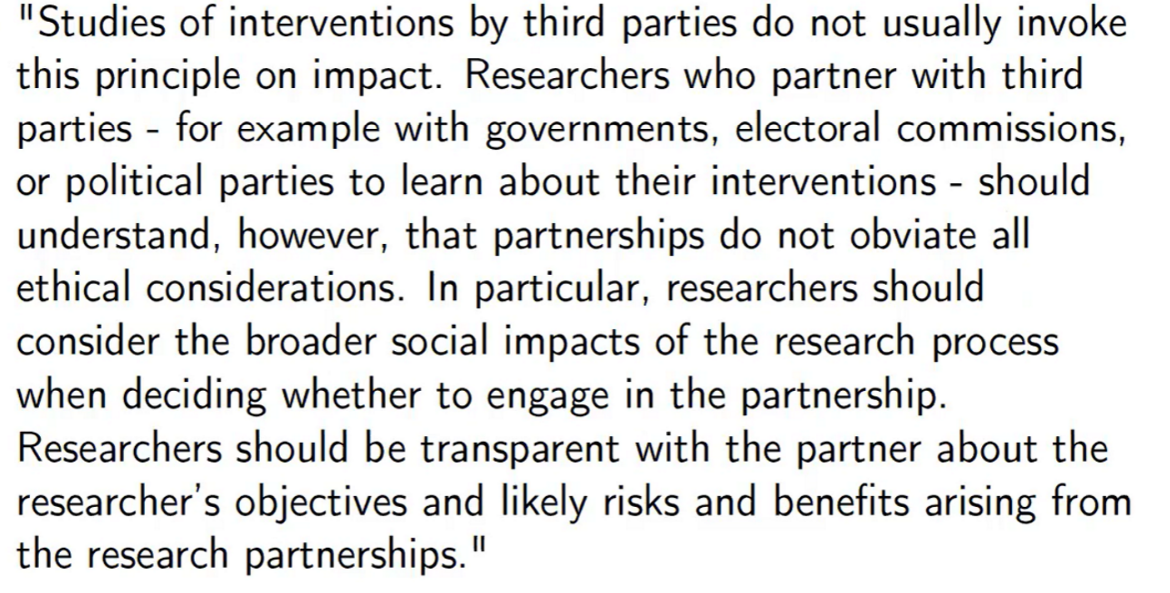
\includegraphics[width=0.8\linewidth]{partnership.png}
    \end{figure}
\end{frame}

\begin{frame}{哪些\textit{不}在伦理考量范围内}
研究完成之后\alert{发布}带来的影响不纳入考量
    \begin{figure}
        \centering
        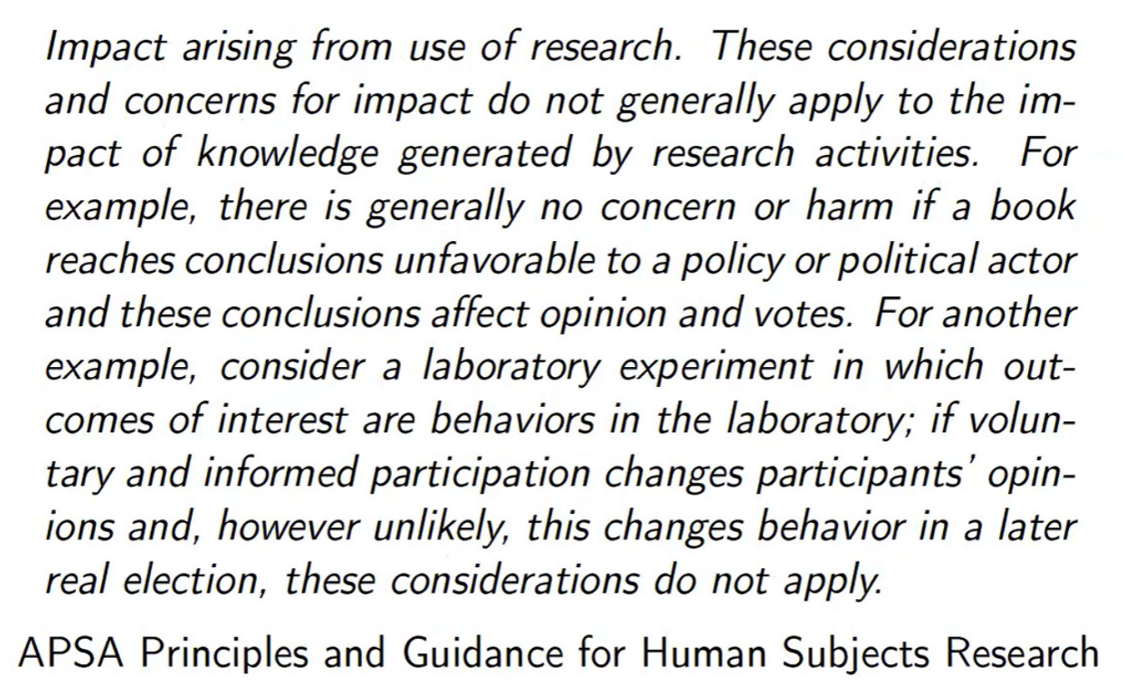
\includegraphics[width=0.9\linewidth]{out.png}
    \end{figure}
\end{frame}

\begin{frame}{不平等权力关系/1}
\begin{itemize}
    \item 在研究的设计和进行过程中，政治科学学者应该明晰研究者和研究对象的\alert{权力差别 power differentials}，以及这种权力不平等可能对“自愿同意”和风险回报分析的影响
    \item 当研究对象在权力结构上是更弱时，研究者要格外注意尊重他们的自主性(autonomy)，保护他们避免受到伤害，以及公平地(fairly)对待研究对象。
    \item 当研究对象在权力结构上更为强势时（比如说官员、机构、公司集团），最低级别以上的伤害以及欺骗行为在某些时候是被允许的。
    \begin{itemize}
        \item 最低级别伤害(minimum harm)：平常人可能在日常生活中遇到的伤害
    \end{itemize}
\end{itemize}
\end{frame}

\begin{frame}{不平等权力关系 /2}
\begin{itemize}
    \item 不平等权力关系在以弱势群体为实验对象时格外突出
    \item 什么导致不平等权力关系？
    \begin{enumerate}
        \item 金钱
        \item 知识
        \item 地位
    \end{enumerate}
\end{itemize}
\end{frame}

\begin{frame}{成本收益计算 Cost-benefit calculation}
\begin{itemize}
    \item 不取得知情同意/欺骗对象的成本大还是这么做的研究收益大？
    \item 取得知情同意/不欺骗对象的成本是什么？
    \item 不取得知情同意的好处有哪些？
    \begin{itemize}
        \item 避免霍桑效应 (Hawthorne effect) $\rightarrow$避免估计偏差
        \begin{itemize}
            \item 研究本身对结果的影响。研究对象知道自己被研究时可能改变他们的行为。可能导致对要研究的影响的误判
        \end{itemize}
        \item 实验更接近现实，构造有效性
    \end{itemize}
\end{itemize}
\end{frame}

\begin{frame}{假想案例 （伦理问题和可能的修改方案）}
\begin{enumerate}
    \item 想研究议员(MPs)是否更少地回应少数民族(ethnic minorities)或者其他党派的支持者。研究者使用随机分配的姓名和党派身份向议员写邮件
    \begin{itemize}
        \item <2->研究不能取得议员同意（否则无意义）
        \item <2->欺骗
        \begin{itemize}
            \item <3->修改：招募少数民族和反对党志愿者
            \item <3->增加成本但是减少了偏差（假身份被发现）
        \end{itemize}
        \item <2->对议员的伤害（名誉）
        \item <2->但是权力关系？
    \end{itemize}
    \item <4->研究发钱(cash transfers)能否阻止东非某国向欧洲的移民。研究者给处理组对象每人发500美元。研究者每两个月跟踪对象，为期两年来测量结果。
    \begin{itemize}
        \item <5->社会-政治结果因为实验过程而改变
        \item <5->不平等权力关系
        \begin{itemize}
            \item <6->如果由第三方合作机构来执行更好
        \end{itemize}
        \item <5->知情同意
        \begin{itemize}
            \item <6->知情同意书
        \end{itemize}
        \item <5->对个体生活的影响
        \begin{itemize}
            \item <6->将控制组安排到一个已有的项目
        \end{itemize}
    \end{itemize}
\end{enumerate}
\end{frame}

\begin{frame}{匿名化：去除个体级别身份识别}
\label{deidentify}
你的发表版本的数据和文章不应该有能识别出对象身份的信息\\
\textbf{目的}：
\begin{itemize}
    \item \alert{保护对象的身份和隐私信息}——一个重要的伦理问题，以及对象的潜在安全问题
    \item 符合法律、IRB和资助者（金主）的要求
\end{itemize}
\end{frame}

\begin{frame}{匿名化/去身份化是什么意思}
\textbf{两种身份识别类型}：
\begin{enumerate}
    \item \alert{直接}：和对象直接挂钩的变量（姓名、邮箱、地址、身份证号、电话号等）
    \item \alert{间接}：几个不同的变量组合起来可以小范围锁定一个人的变量（性别、出生日期、其他特别日期、地理信息、罕见职业、教育经历等）
\end{enumerate}
数据识别性不是二元binary的（不是能识别/不可识别），而是一个连续的变量。详见下图
\end{frame}

\begin{frame}{图片来源:\href{https://fpf.org/wp-content/uploads/2016/04/FPF_Visual-Guide-to-Practical-Data-DeID.pdf}{链接}}
\begin{figure}
    \centering
    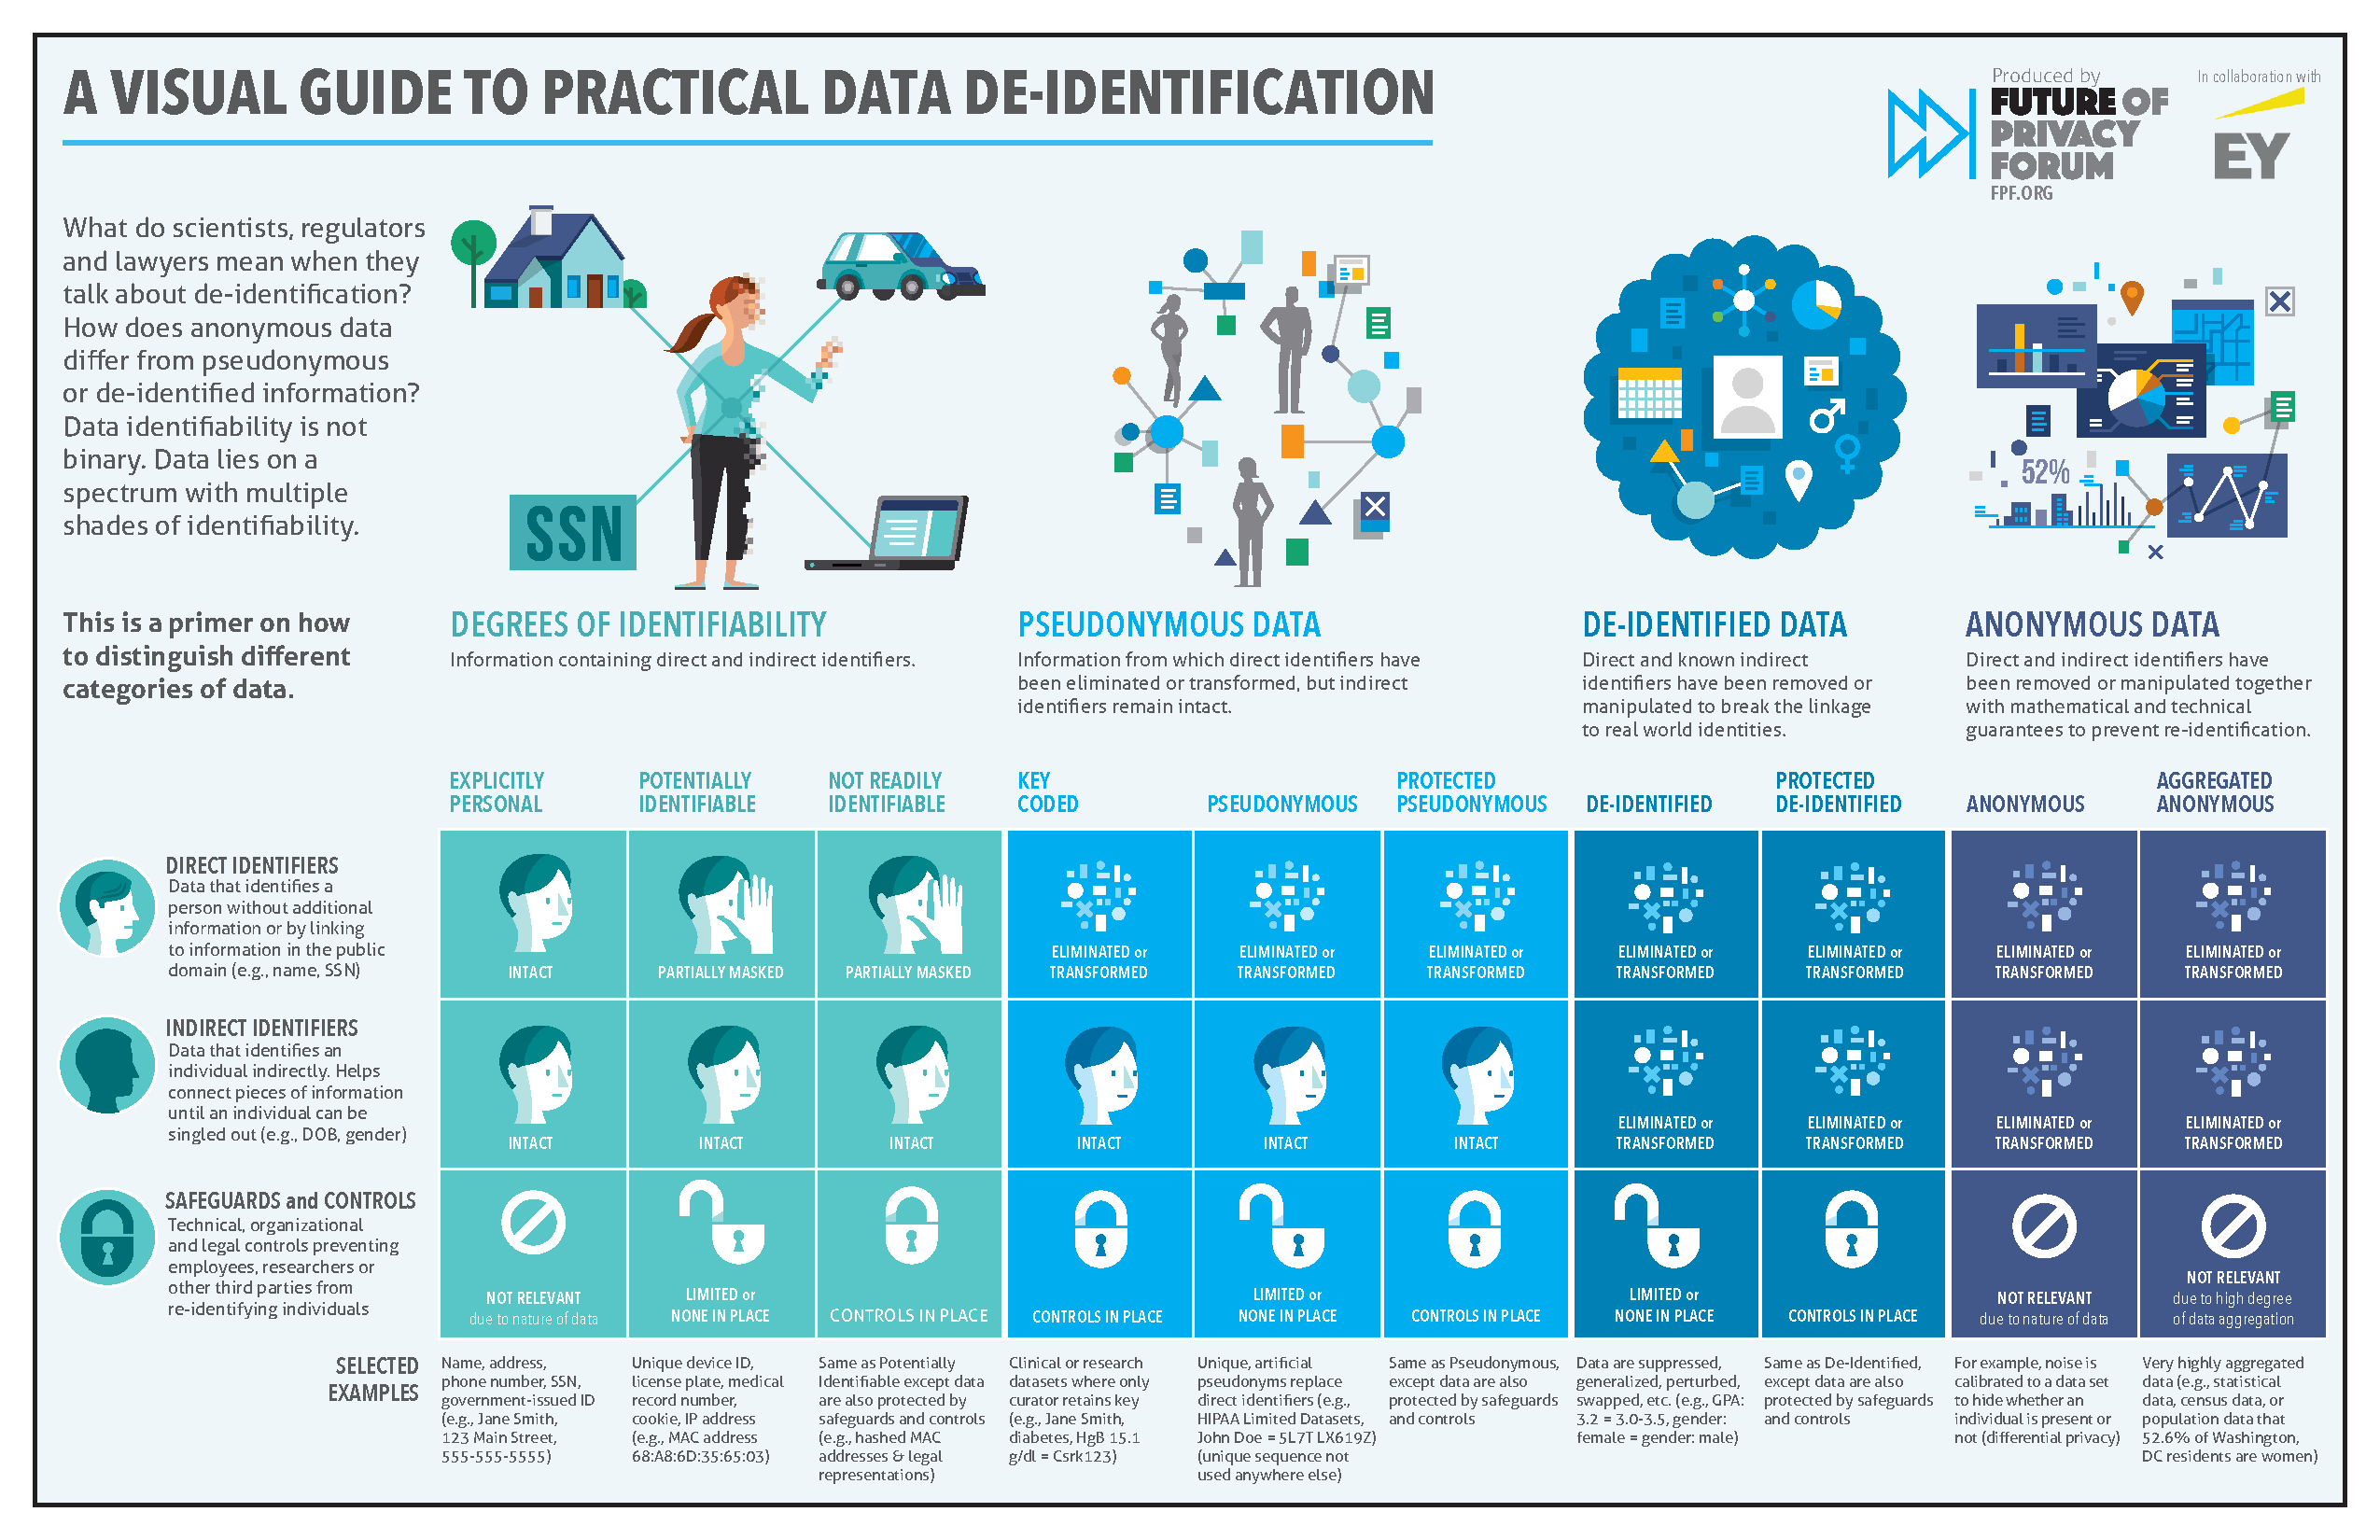
\includegraphics[width=\linewidth]{identifiability.pdf}
\end{figure}
\end{frame}

\begin{frame}{间接识别特征(identifiers)的例子}
\begin{itemize}
    \item 你的调查问卷采集了老师的\textbf{性别}、\textbf{所教年级}和\textbf{年龄}的信息
    \item 如果在这个学校的三年级老师中只有一位女老师年龄在40-49岁区间，那么她在你的数据里就相当于是\alert{实名}的.
    \item 生日（年月日）、性别、邮编能够准确定位美国87\%的人. (\cite{sweeney2000})
\end{itemize}
\end{frame}

\begin{frame}{例：使用健康数据的人肉攻击 (\cite{Emam2011})}
\begin{figure}
    \centering
    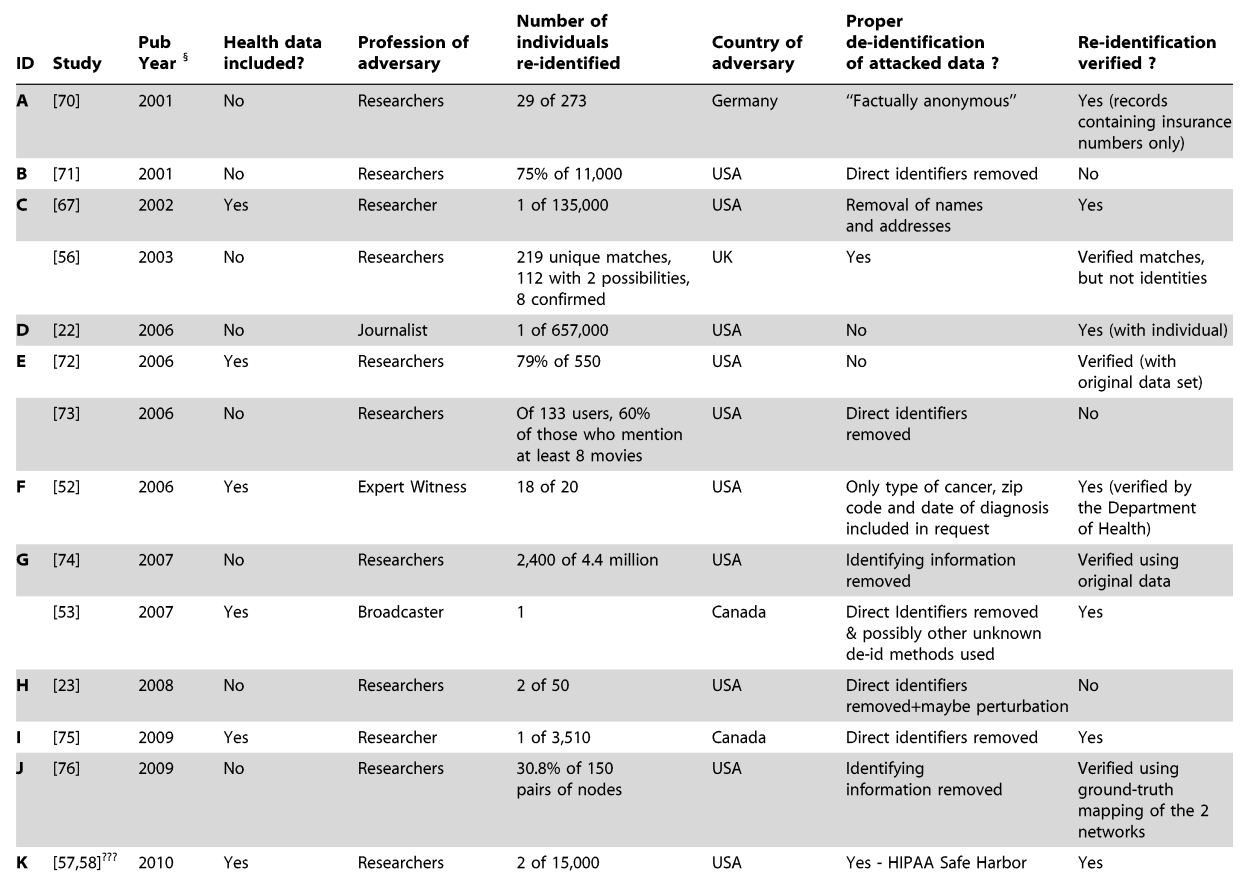
\includegraphics[width=0.9\linewidth]{identattack.png}
\end{figure}
\end{frame}

\begin{frame}{对于直接识别变量(direct identifiers)的处理}
通常来讲，直接识别变量，比如说姓名、地址、手机号、身份证号，\alert{永远}不要公布。\\
\textbf{选项}：
\begin{itemize}
    \item 将这些变量移出公开数据
    \item 使用伪造信息(Pseudonymize)。
    \begin{itemize}
        \item 可逆的(reversible)：一一对应
        \item 不可逆(reversible): 随机分配
    \end{itemize}
\end{itemize}
\end{frame}

\begin{frame}{图片展示：}
\begin{figure}
    \centering
    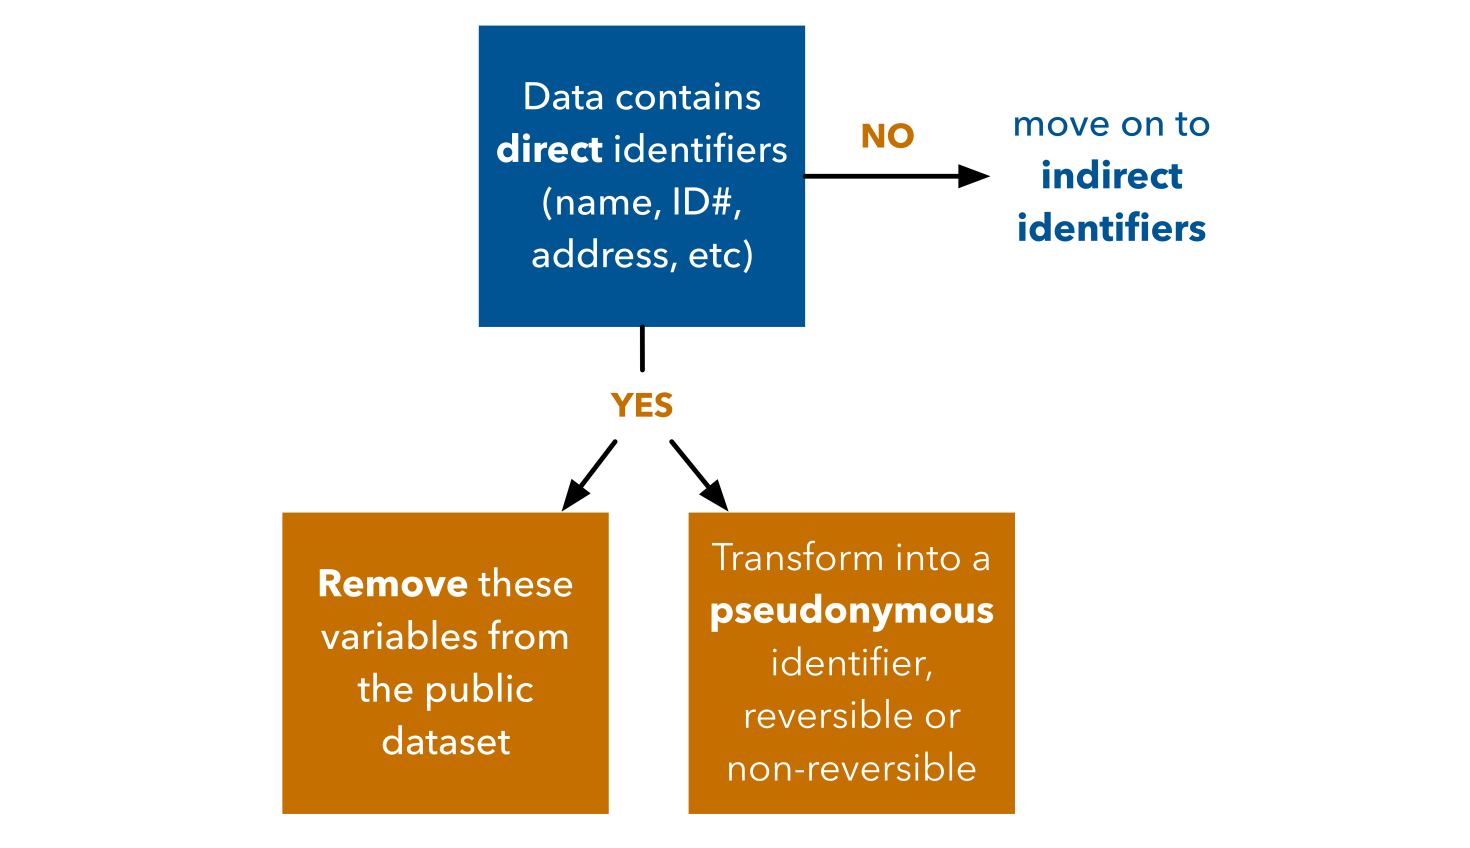
\includegraphics[width=0.9\linewidth]{pseudonymize.png}
\end{figure}
\end{frame}

\begin{frame}{对于间接识别特征我们需要做到什么程度呢？}
\begin{enumerate}
    \item \textbf{确定风险程度}：$Pr(\text{识别出来})\times$敏感程度
    \item \textbf{选择'k-匿名'程度(k-anonymous level)}: 每一个记录都从至少$k-1$个其他人中无法分辨
    \item \textbf{选择合适的去身份化(de-identification)方法}:汇总数据、移出特定变量和观察值、减少信息、在数据中加入随机值或者噪音(noise).
\end{enumerate}
\end{frame}

\begin{frame}{例：k=3时的k-匿名度}
\begin{figure}
    \centering
    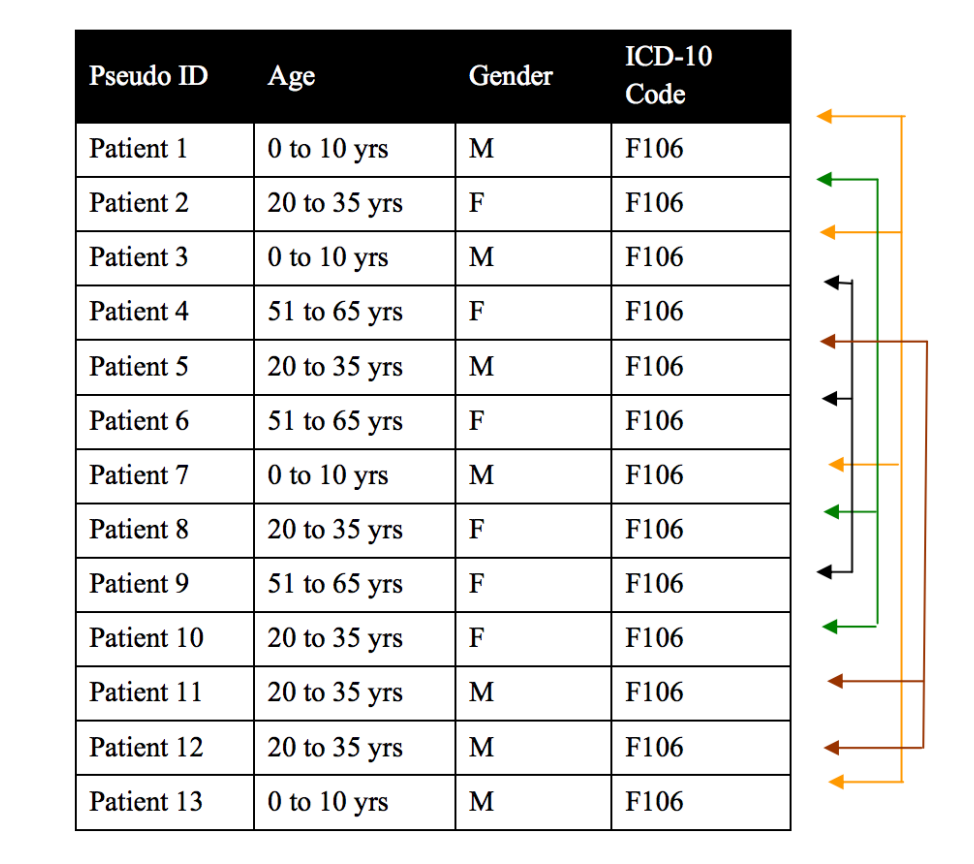
\includegraphics[width=0.7\linewidth]{kanonymous.png}
\end{figure}
\end{frame}

\begin{frame}{图片展示：间接识别特征的解决方案}
\begin{figure}
    \centering
    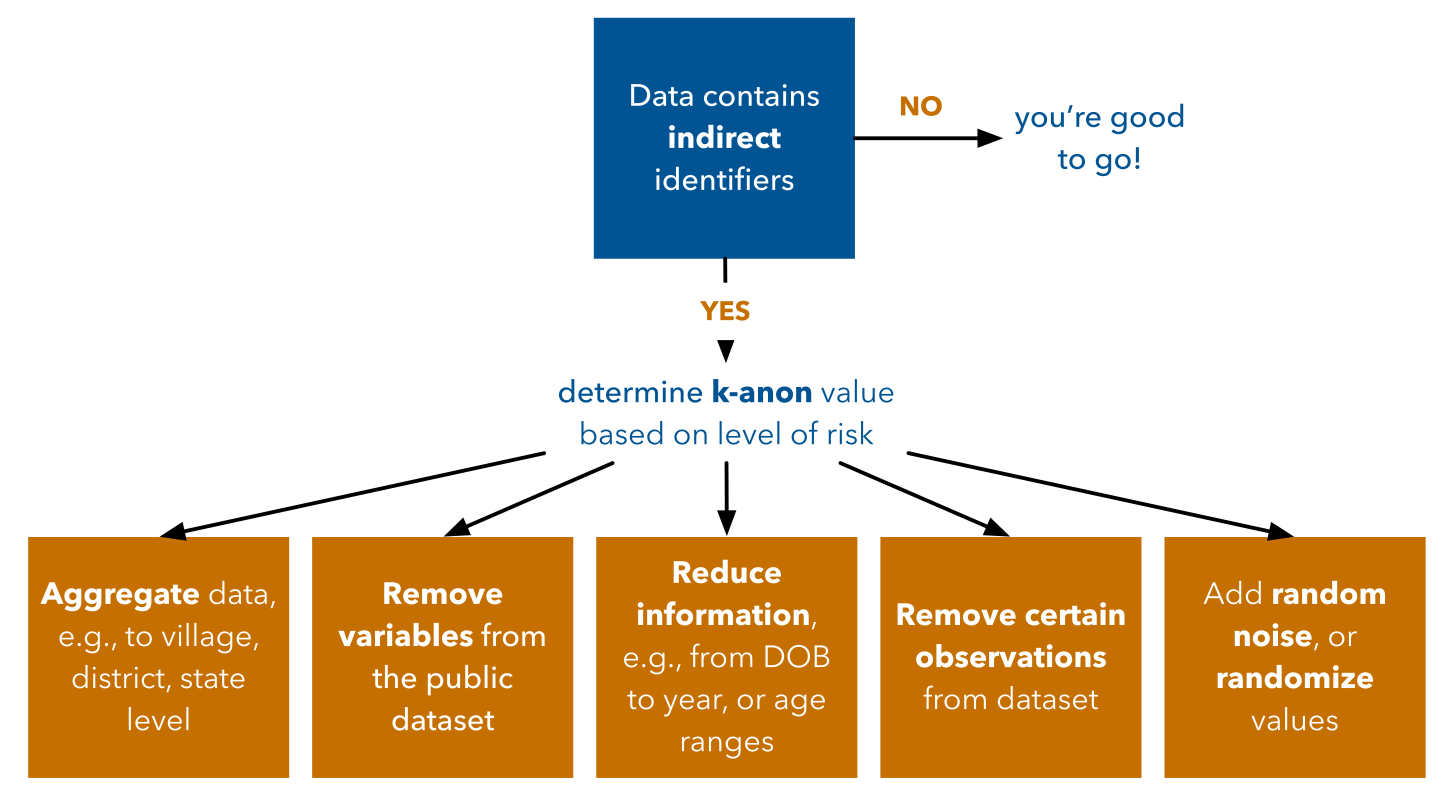
\includegraphics[width=0.9\linewidth]{indirect.png}
\end{figure}
\end{frame}

\begin{frame}{取舍：有用(usefulness)$\Longleftrightarrow$匿名性(anonymity)}
\begin{itemize}
    \item \textbf{汇总数据} - 失去个人-层面分析的\alert{可复现性}replicability.
    \item \textbf{移除变量} - 有可能不能复现某些模型设定
    \item \textbf{移出观察} - 如果非随机的话会产生偏差bias+失去精确度
    \item \textbf{减少变量信息} - 增加模型的噪音(noise)$\Rightarrow$失去精确度
    \item \textbf{增加随机噪音}/值 - 增加噪音失去精确度
\end{itemize}
更多关于匿名化门槛、方法和工具的讨论：\href{http://www.ehealthinformation.ca/wp-content/uploads/2014/08/2010-Risk-based-de-identification-of-health-data.pdf}{链接1} \href{http://www.ehealthinformation.ca/wp-content/uploads/2014/08/2009-Tools-for-De-Identification-of-Personal-Health.pdf}{链接2}
\end{frame}

\begin{frame}{清洗含有身份特征数据时的行为规范}
\begin{itemize}
    \item \alert{保留}所有处理/分析含有身份特征数据的代码，除非代码本身危害到了匿名性
    \begin{itemize}
        \item 比如说，用来生成随机姓名/身份证号码的\textbf{随机数种子}代码要删掉
    \end{itemize}
    \item 如果含有身份特征的数据\alert{没有}用于分析，那么尽早在数据清洗阶段就把这些变量删掉
    \item 安全地存放原数据（含有身份特征的数据）
\end{itemize}
\end{frame}

\section{分析阶段的学术规范}
\label{phaseII}
\begin{frame}{分析阶段的学术规范}
“\textbf{Reproducibility} 可再现性 is just collaboration with people you don't know, includuing yourself next week” - Philip Stark, UC Berkeley
\begin{figure}
    \centering
    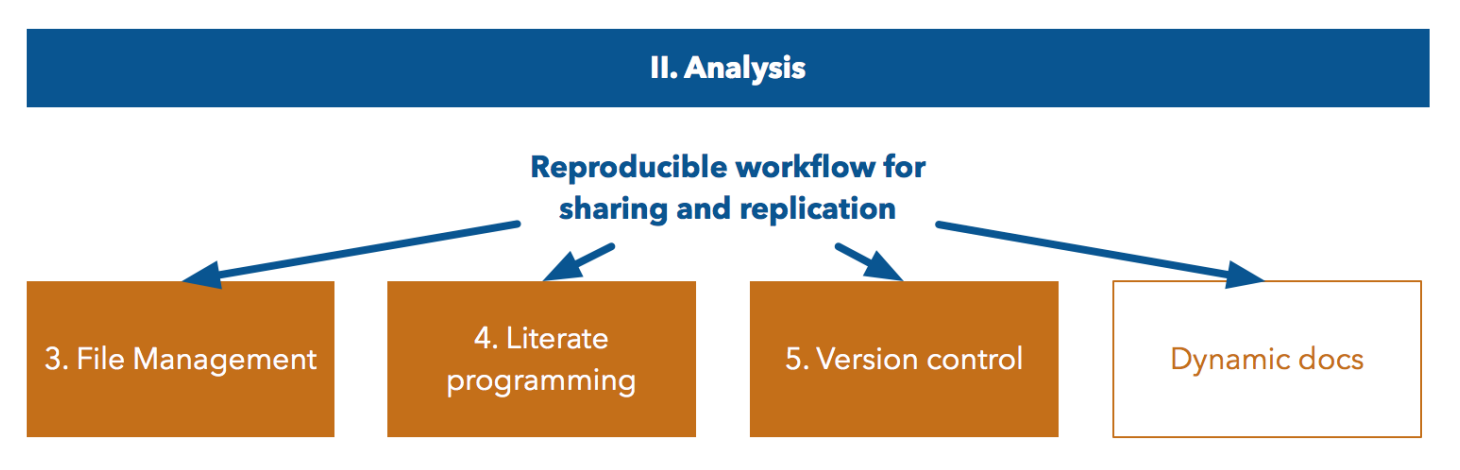
\includegraphics[width=0.9\linewidth]{analysis.png}
\end{figure}
\end{frame}

\begin{frame}{文件管理 File Management}
\begin{itemize}
    \item \textbf{定义}：指的是整洁地(cleanly)和直觉地(intuitively)组织和管理你的文件
    \item \textbf{原因}： 保存原数据(original data)、简化工作流程、减少分享文件时的准备时间
\end{itemize}
\end{frame}

\begin{frame}{反例：别搞成这样}
\begin{figure}
    \centering
    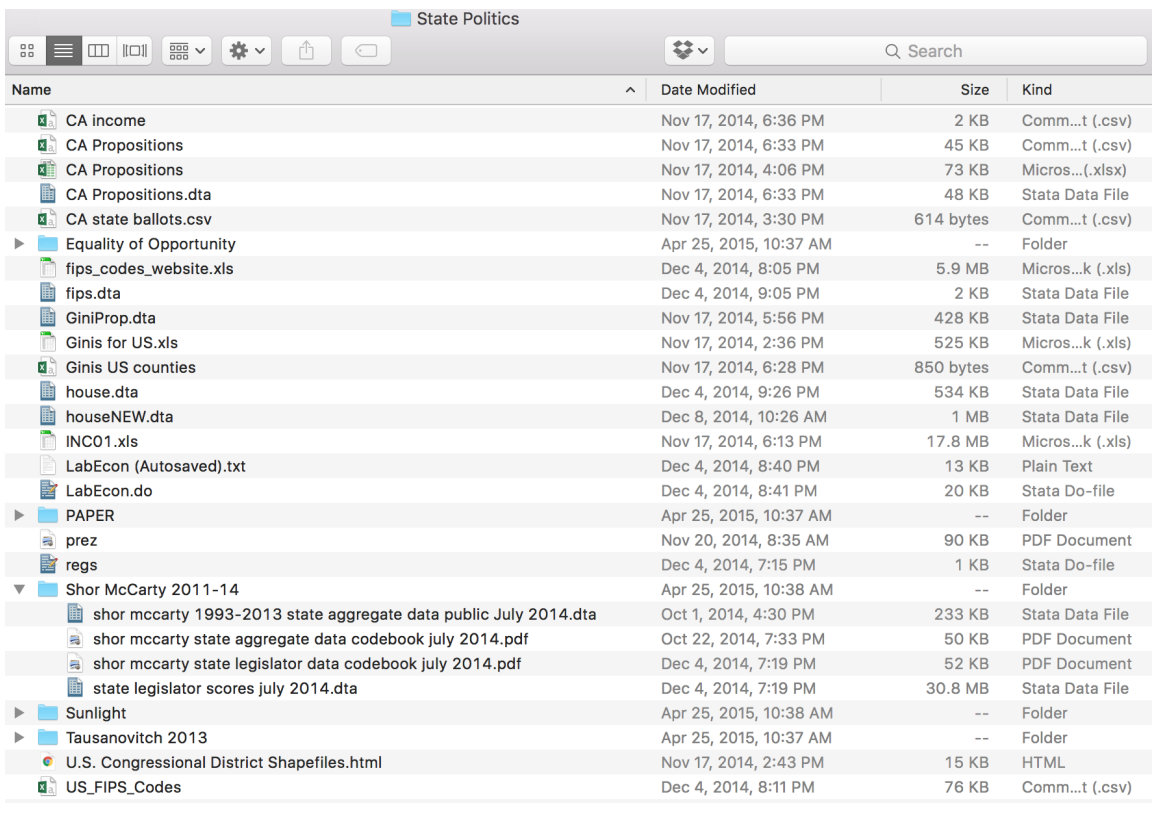
\includegraphics[width=0.9\linewidth]{messy.png}
\end{figure} 
\end{frame}

\begin{frame}{最好使用PDEL（或类似的）模板}
下载地址：\url{https://github.com/PolicyDesignEvaluationLab/Transparency-Initiative}
    \begin{figure}
    \centering
    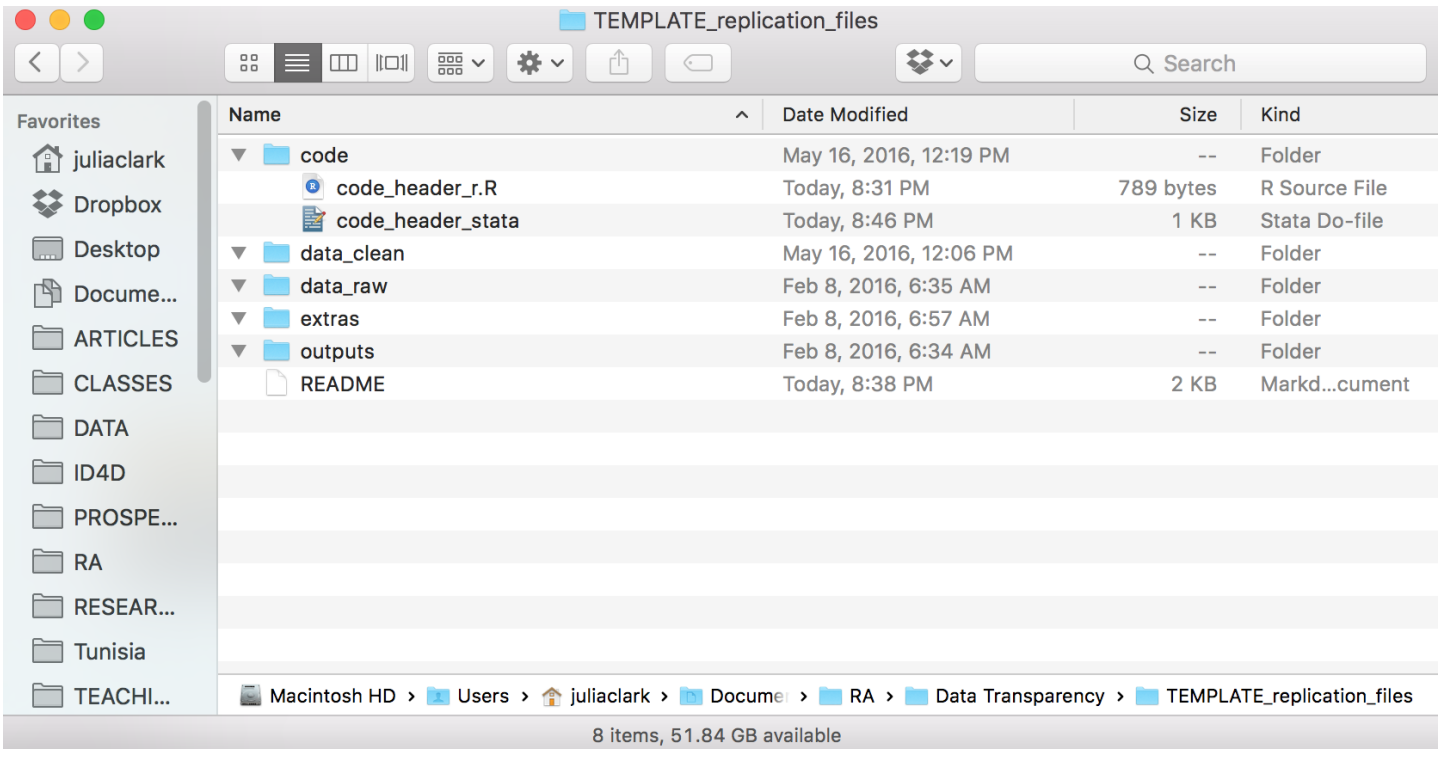
\includegraphics[width=0.9\linewidth]{PDEL.png}
\end{figure} 
\end{frame}

\begin{frame}{编程可读性 Literate Programming}
\begin{itemize}
    \item \textbf{定义}：保证我们的代码对于\textit{人类}是好理解的
    \item \textbf{原因}： 为了别人能更好地复现我们的结果；也帮助我们自己避免错误
\end{itemize}
\end{frame}

\begin{frame}{他好我也好}
    \begin{figure}
    \centering
    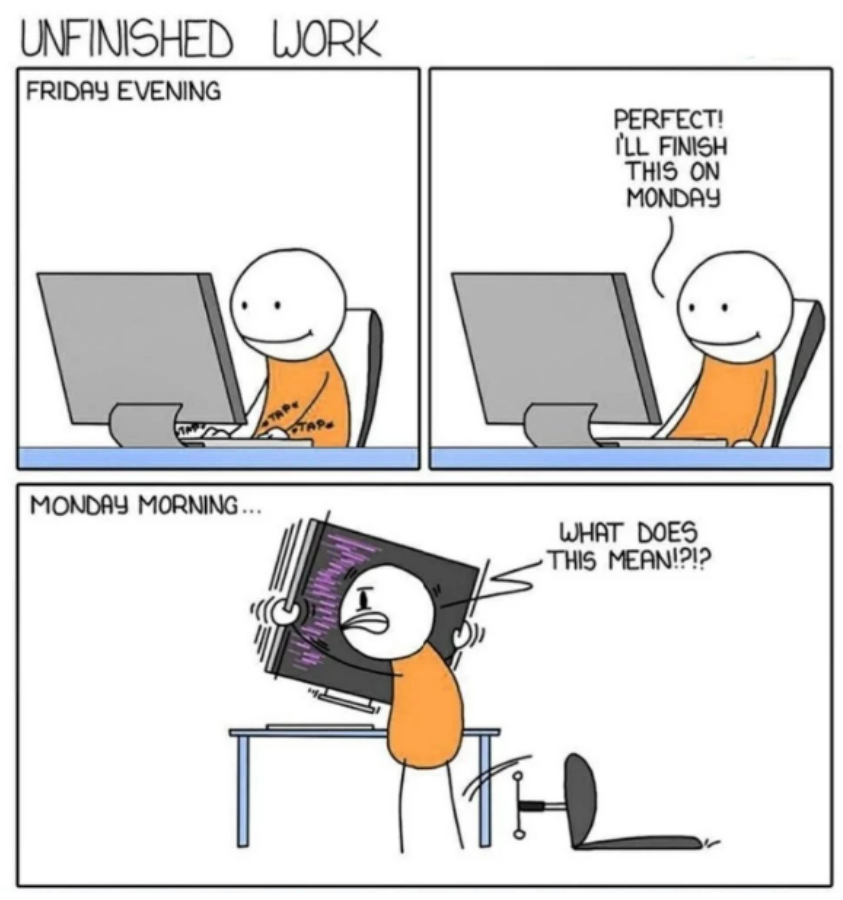
\includegraphics[width=0.6\linewidth]{unfinishedwork.png}
    \end{figure}
\end{frame}

\begin{frame}{基本准则}
\begin{itemize}
    \item 符合直觉地给文件分组/取名
    \item 让没接触过你研究的人也能找到对应的代码/数据/图标产出
    \item 简化代码避免重复
\end{itemize}
\end{frame}

\begin{frame}{文件分组/命名}
\begin{itemize}
    \item 将数据清洗/合并(cleaning/merging)的代码和数据分析(data analysis)的代码分开，并写一个主脚本(master-script)能够同时运行两者
    \item 为代码、数据文件和产出取符合逻辑的名字
    \begin{itemize}
        \item 把代码文件(scripts)以运行顺序编号(e.g. \texttt{1\char`_main\char`_analysis.R}, \texttt{2\char`_robust\char`_checks.R})
        \item 以描述性的名字命名产出(output)文件，因为编号可能改变(比如说\texttt{figure\char`_hte.png}就要比\texttt{figure\char`_1.png}要好)
    \end{itemize}
\end{itemize}
\end{frame}

\begin{frame}{改善索引(navigation)}
\begin{itemize}
    \item 在代码开头撰写描述(headers).
    \begin{itemize}
        \item 使用'\#'写注释
    \end{itemize}
    \item 把代码整理成易读的格式
    \begin{itemize}
        \item 结构
    \end{itemize}
    \item 增加注释帮助理解
    \item 分段：主分析、产出...
    \item 给函数、对象(objects)、变量(variable)取符合直觉的名字
    \begin{tabular}{|c|c|}
    \hline
       \texttt{edu\char`_percent}  & √ \\ \hline
       \texttt{v76}  & × \\ \hline
    \end{tabular}
\end{itemize}
\end{frame}

\begin{frame}{页首描述 (header) 范例}
\begin{figure}
    \centering
    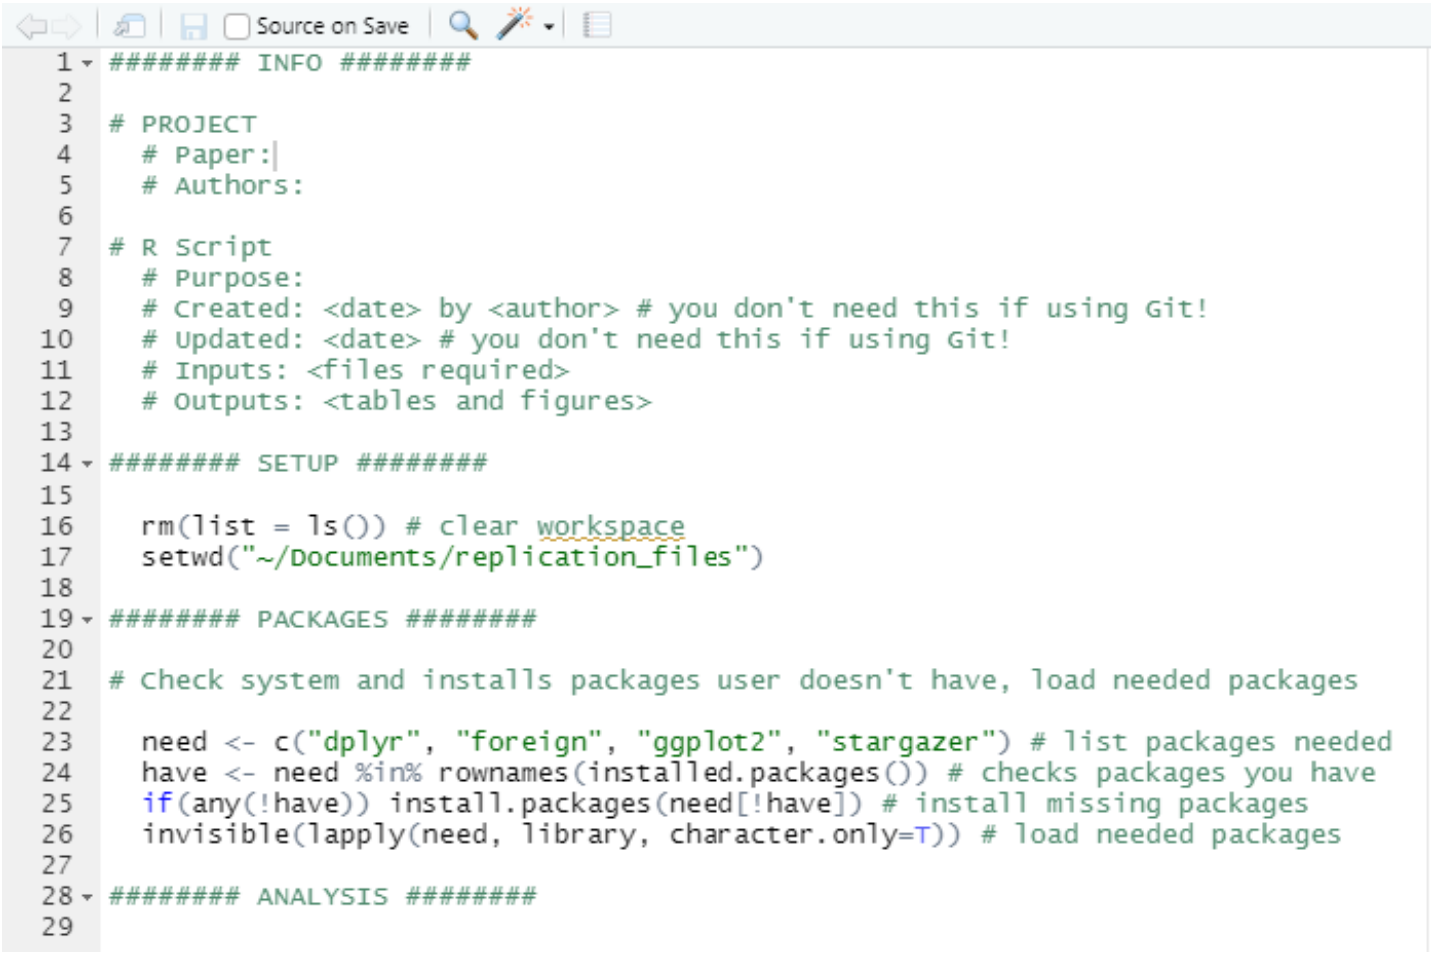
\includegraphics[width=0.9\linewidth]{header.png}
    \end{figure}
\end{frame}

\begin{frame}{简化代码：设置工作目录(working directories)}
\textbf{R:} \texttt{setwd("∼/Documents/replication\char`_files")} \\
\textbf{Stata:} \texttt{capture cd "∼/Documents/replication\char`_files"}
\begin{itemize}
    \item 节省时间：因为复现你代码的人只用改变这行代码一次就能调整工作目录
    \item 特别是对于苹果Mac系统('\char`/')和Windows系统('\char`\\')交替使用的人来说格外有用
\end{itemize}
不过我们的代码更为先进：将工作目录设为文件目录：\\
\texttt{setwd(dirname(rstudioapi::getSourceEditorContext()\$path))
}
\\~\\
如果代码文件在\texttt{code}文件夹里，而想把工作目录设为上级目录，可以使用：\\
\texttt{setwd(gsub("/code","",dirname(rstudioapi::\\getSourceEditorContext()\$path)))
}
\end{frame}

\begin{frame}{版本控制 Version Control}
\begin{figure}
    \centering
    
\includegraphics[width=0.5\linewidth]{versionctrl.png}
\end{figure}
\end{frame}

\begin{frame}{关于版本控制}
\begin{itemize}
    \item \textbf{定义}：一个用来管理不同时间和不同合作者collaborators间\alert{迭代的}iterative文件（代码、数据、草稿manuscripts）的系统。
    \item \textbf{原因}：保存原文件、保护成果、合作效率、简化工作流程
\end{itemize}
\end{frame}

\begin{frame}{版本控制的原则}
\begin{itemize}
    \item 储存好原数据（不要在原数据上有任何更改）
    \item 对文件的改变要有记录(documented)，确保可逆(reversible.
    \item 将“主要”(master)版本的文件按照工作顺序(working order)存放，在做试验调整(experimenting)之前留好备份
    \item 对于不同贡献者的更改要做好调和(reconcile).
\end{itemize}
\end{frame}

\begin{frame}{操作方案 Manual Solutions}
\begin{itemize}
    \item 为每个主要变动保留含有日期的副本
    \item 对于每一个变动，都重新跑一遍所有的代码保证没有“损坏”
    \item 和其他作者(co-authors)打好招呼，确保大家不在同时对同样的文件进行编辑
    \item 通过写日志(log)来提醒自己主要变动的位置/内容/日期。
\end{itemize}
\end{frame}

\begin{frame}{版本控制软件 > Git > GitHub}
你也可以让\alert{版本管理软件(version control software)}为你做上述的事情
\begin{itemize}
    \item \textbf{版本管理软件：}帮助管理版本/文件的编辑（很多选项）
    \item \textbf{Git:} 开源、“分布式模型”的版本控制
    \item \textbf{GitHub:}基于 Web 的免费服务，托管 Git“存储库”并提供各种协作功能
\end{itemize}
GitHub能解决以下常见问题：
\begin{itemize}
    \item \textbf{追踪(tracking)代码/文本里的变化：}谁在什么时间在哪改变了什么
    \item \textbf{选择性的回退(reverting changes):}比简单的撤销\texttt{ctrl + Z}来的强大
    \item \textbf{实验：}比"my\_code\_v2\_new.R"来得方便
    \item \textbf{合作:}分享/审查(vetting)/协调(reconciling)变化
\end{itemize}
\end{frame}

\begin{frame}{Git资源}
太多了，只选取一些讲讲：
\begin{itemize}
    \item \href{http://www.chronicle.com/blogs/profhacker/a-gentle-introduction-to-version-control/23064}{对萌新友好的版本控制入门}
    \item \href{https://www.hastac.org/blogs/harrisonm/2013/10/12/github-academia-and-collaborative-writing}{GitHub和学术界的合作式写作}
    \item \href{http://www.chronicle.com/blogs/profhacker/forks-and-pull-requests-in-github/47753}{分叉(forks)和拉取请求(pull requests)}
    \item \href{http://blog.scottlowe.org/2015/01/14/non-programmer-git-intro/}{非程序员使用Git命令行的介绍}
    \item \href{http://blog.scottlowe.org/2015/01/27/using-fork-branch-git-workflow/}{使用命令行(command line)的分支(Fork-branch)工作流程（但对于图形界面使用者也很有用）}
\end{itemize}
\end{frame}

\begin{frame}{动态文档 Dynamic Docs}
你可以进一步地深化可复现研究的观念：使用\href{http://rmarkdown.rstudio.com/}{RMarkdown}整合你的代码和文章草稿(manuscript)
\begin{figure}
    \centering
    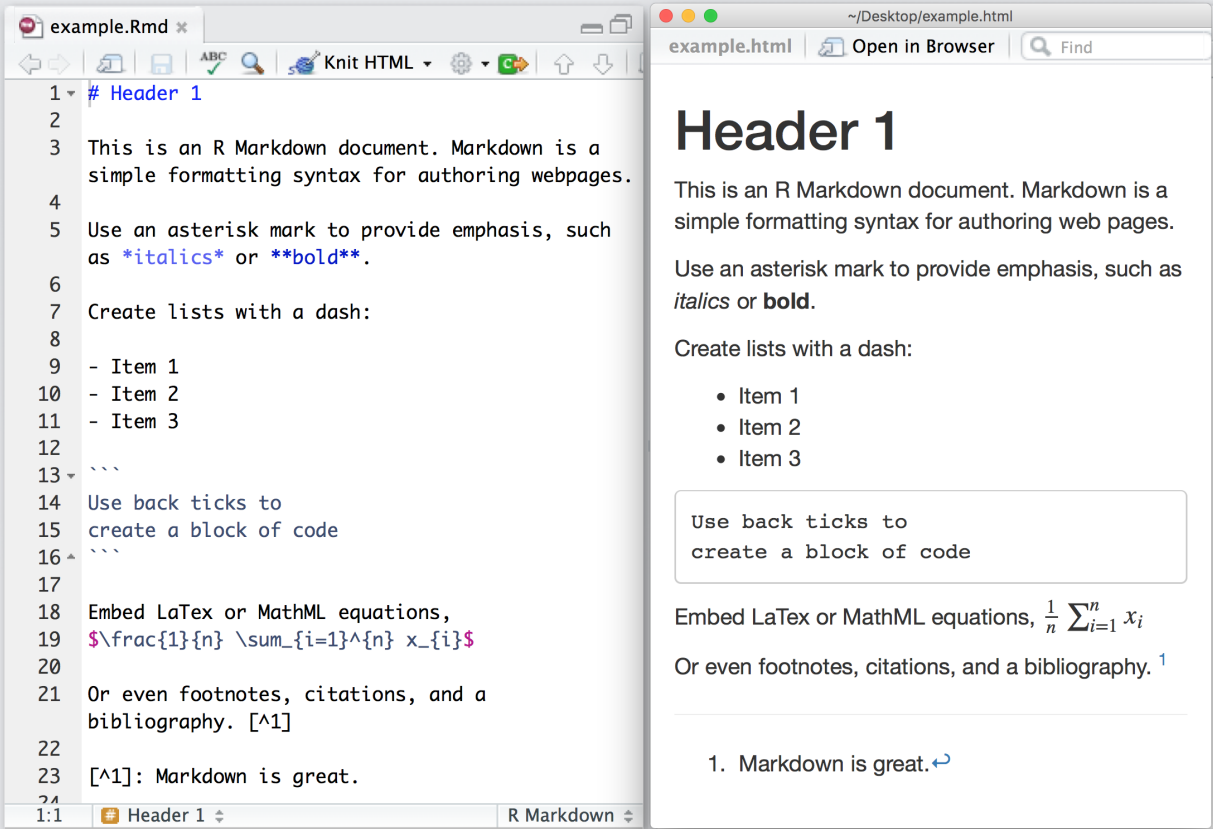
\includegraphics[width=0.8\linewidth]{rmarkdown.png}
\end{figure}
\end{frame}

\section{传播(Dissemination)阶段的学术规范}
\begin{frame}{传播(Dissemination)阶段的学术规范}
\begin{figure}
    \centering
    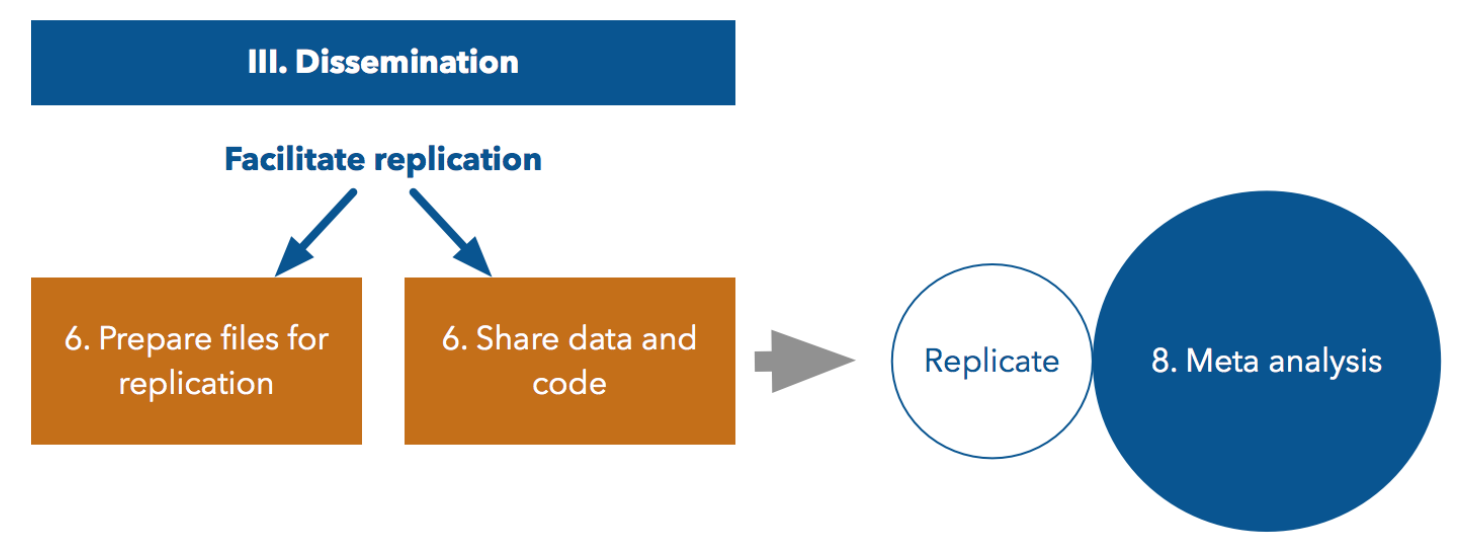
\includegraphics[width=\linewidth]{dissemination.png}
\end{figure}
\end{frame}

\begin{frame}{为什么我们要让代码可复现呢？}
\begin{itemize}
    \item \textbf{利他原因：}科学过程的一部分，同时也是公共商品(public good)
    \item \textbf{利己原因：}让代码更好的为己所用，减少因为错误而现大眼的几率，增加自己研究的透明度和可信度
\end{itemize}
\end{frame}

\begin{frame}{复现文件应该...}
\begin{itemize}
    \item 是完整且精简(parsimonious)的
    \item 能够一键运行和生成所有结果
    \item 对于人类是可读(readable)且易于解读(interpretable)的
    \item 保护个人信息隐私的
\end{itemize}
\textbf{警告：}对于整理复现文件没有单一“最好的”方法。用适合你的就好（只要符合以上标准）
\end{frame}

\begin{frame}{准备复现文件的五个步骤}
\begin{enumerate}
    \item \hyperlink{setup}{设置 Set-up}
    \item \hyperlink{ini.rep}{初步复现 Initial replication}
    \item \hyperlink{deidentify}{去身份化 De-identify}
    \item \hyperlink{clarity}{编辑 Edit}
    \item \hyperlink{final.rep}{最终复现 Final replication}
\end{enumerate}
\end{frame}

\label{setup}
\begin{frame}{1. 设置 Set-up}
创造一个新的、组织整洁的复现文件夹，有选择地将文件加到里面 \\
\textbf{目的：}
\begin{itemize}
    \item 保证文件是\alert{完整、精简且易读的}
    \item 保护源文件
\end{itemize}
\end{frame}

\begin{frame}{设置复现文件}
新建以下文件/目录：
\begin{enumerate}
    \item 在你的项目目录\textit{内}新建\textbf{一个新的、空的复现文件夹}(e.g. "\texttt{replication\char`_files/}")
    \item 子文件夹(subfolders):
    \begin{itemize}
        \item \texttt{code/}--代码(scripts)
        \item \texttt{data\char`_clean/} -- 已清洗数据(manipulated data)
        \item \texttt{data\char`_raw/} --原数据
        \item \texttt{output/} -- 创造的图表等
        \item \texttt{extra/} -- 其他的(misc)文件(e.g. code book密码本)
    \end{itemize}
    \item \textbf{一个"README.txt"文件} 来记录目录、来源、软件/系统版本、（电脑型号信息）、以及其他复现/理解所需要的信息
\end{enumerate}
\end{frame}

\begin{frame}{2. 初步复现 Initial Replication}
\label{ini.rep}
\textit{复制}(不要移动)数据和代码文件到刚创建的复现文件夹，然后\alert{尝试复现你的结果}。\\
~\\
\textbf{目的}：
\begin{itemize}
    \item 在整理结构和格式之前确保你的代码可以运行且\alert{复现}你的结果
    \item 确保复现文件夹的数据/代码文件是\alert{完整且精简的}
    \begin{itemize}
        \item 有且只有相关文件
    \end{itemize}
\end{itemize}
\end{frame}

\begin{frame}{A. 检查分析 (Check Analysis)}
通常来讲，先从最后的数据分析开始检查，然后反向往最初的数据清洗/合并的阶段进行更为容易。
\begin{enumerate}
    \item 将原始的数据分析代码(analysis scripts)复制至\texttt{replication\char`_files/code}目录
    \item 将用于分析的清洗之后的数据复制至\texttt{replication\char`_files/data\char`_clean}目录
    \item （除了工作目录wd）不加任何更改地运行代码
    \item 修复出现的bugs,处理任何和之前结果不一样的差异(discrepancies)
\end{enumerate}
\end{frame}

\begin{frame}{B. 检查数据清理/合并 (data clean/merge)}
\begin{enumerate}
    \item 如果数据分析设数据清理不在一起，先把数据清理/合并的代码复制至\texttt{replication\char`_files/code}目录
    \item 将原数据复制至\texttt{replication\char`_files/data}目录
    \item （除了工作目录wd）不加任何更改地运行数据清理/合并代码
    \item 如果我们得到的结果（数据）文件和步骤A里的已清理数据不一样，说明数据清理数据里面有纰漏，需要修复。
\end{enumerate}
\end{frame}

\begin{frame}{3. 个人级别(individual-level)数据的去身份化}
如果你还没有去身份化的话，请参照之前的\hyperlink{deidentify}{说明}进行操作
\end{frame}

\begin{frame}{4. 清晰地编辑/组织文件 Edit and Organize Files for Clarity}
\label{clarity}
下一步则是清洗并标注数据、代码和其他文件来增加可用性(usability). \\~\\

\textbf{目的：}
\begin{itemize}
    \item 保证文件在结构和内容上是\alert{清晰易读(legible)}的
\end{itemize}
\end{frame}

\begin{frame}{基本步骤}
\begin{itemize}
    \item 为文件命名、按结构存放*
    \item 简化(streamline)并注释(annotate)代码*
    \item 将文件和文件夹内容记录在册(README文件)
\end{itemize}
\alert{*如果你按照之前\hyperlink{phaseII}{第二阶段}可读编程的建议操作的话，这两步不用额外操作}
\end{frame}

\begin{frame}{记录文件和文件夹内容信息}
\begin{itemize}
    \item 在README文件里添加关于replication目录和内容的信息
    \item 如果需要的话，在"\texttt{extra/}"文件夹里加入密码本(code book)
    \item 在README文件里添加所用的支持库(packages)和软件版本信息
    \begin{itemize}
        \item \textbf{R:}\texttt{sessionInfo()}
        \item \textbf{Stata:}\texttt{version}
    \end{itemize}
\end{itemize}
\end{frame}

\begin{frame}{5.最终复现 Final Replication}
\label{final.rep}
\begin{itemize}
    \item 关闭或者清理你的Stata/R/etc.工作环境(memory)
    \begin{itemize}
        \item 重启软件并Restart session
    \end{itemize}
    \item 重新运行整个过程 - 数据合并、清洗和分析 - 从而确保我们的编辑没有影响到正常运行
    \item 在一个朋友(或者研究助理RA)的电脑上跑一遍作为最终检查
    \begin{itemize}
        \item 在不同系统(Windows, Mac OS)和不同平台(Intel, Apple, AMD)上测试最佳
    \end{itemize}
    \item 确保测试一致之后，文件可以被发布/分享
\end{itemize}
\end{frame}

\begin{frame}{分享数据和代码}
\begin{itemize}
    \item 具体来讲，只在一个在线存储库(repository)上传复现文件
    \item \textbf{原因：}在线存储库比个人网站存放更久、更容易被搜到，可以在未来作为证据
    \item \textbf{一些问题/担忧：}
    \begin{itemize}
        \item 有时候会被延迟发布(embargoed)，或者只提供复现相关的文件(e.g. 没有用到的调查问卷问题不予发布)
        \item 最大的风险不是数据/想法被盗，而是研究受到忽视(\cite{King95})
        \item 如果版权受限(proprietary)则很难公开数据
    \end{itemize}
\end{itemize}
\end{frame}

\begin{frame}{在哪共享数据呢}
取决于学科：你可以通过\url{http://www.re3data.org/}查找你学科常用的在线存储库，或者尝试以下常用选项：
\begin{itemize}
    \item 最著名的: \href{https://dataverse.harvard.edu/}{\textbf{Harvard Dataverse}}
    \item \href{https://osf.io/}{Open Science Framework}
    \item \href{https://www.openicpsr.org/openicpsr/}{OpenICPSR}
\end{itemize}
\end{frame}

\begin{frame}{元分析 Meta-Analysis}
\begin{itemize}
    \item \textbf{定义：}对于一组\alert{研究结果本身}的统计分析，以得出处理效果的\alert{汇总估计}(pooled estimate)，或者进行\textbf{系统性回顾}(systematic review)。
    \item \textbf{原因：}单个研究的估计值可能是\alert{有偏的}(biased)或者存在\alert{随机误差}(random error)
    \begin{itemize}
        \item 重点假设：没有\alert{出版偏差}(publication bias)
    \end{itemize}
\end{itemize}
\end{frame}

\begin{frame}{一个研究$=$一个数据点(Data Point)}
哪怕一个研究有3,685名对象参与实验，对于元分析来说，也只是众多研究当中的一个数据点(data point)
\begin{itemize}
    \item 结果可能是小概率事件(random chance)吗？
    \item 样本是否有偏差(bias)？
    \item 如果另一个研究者分析了你的数据，结果是否会不同？
\end{itemize}
\end{frame}

\begin{frame}{哪怕使用相同的数据，结果也可能会不同...}
\begin{figure}
    \centering
    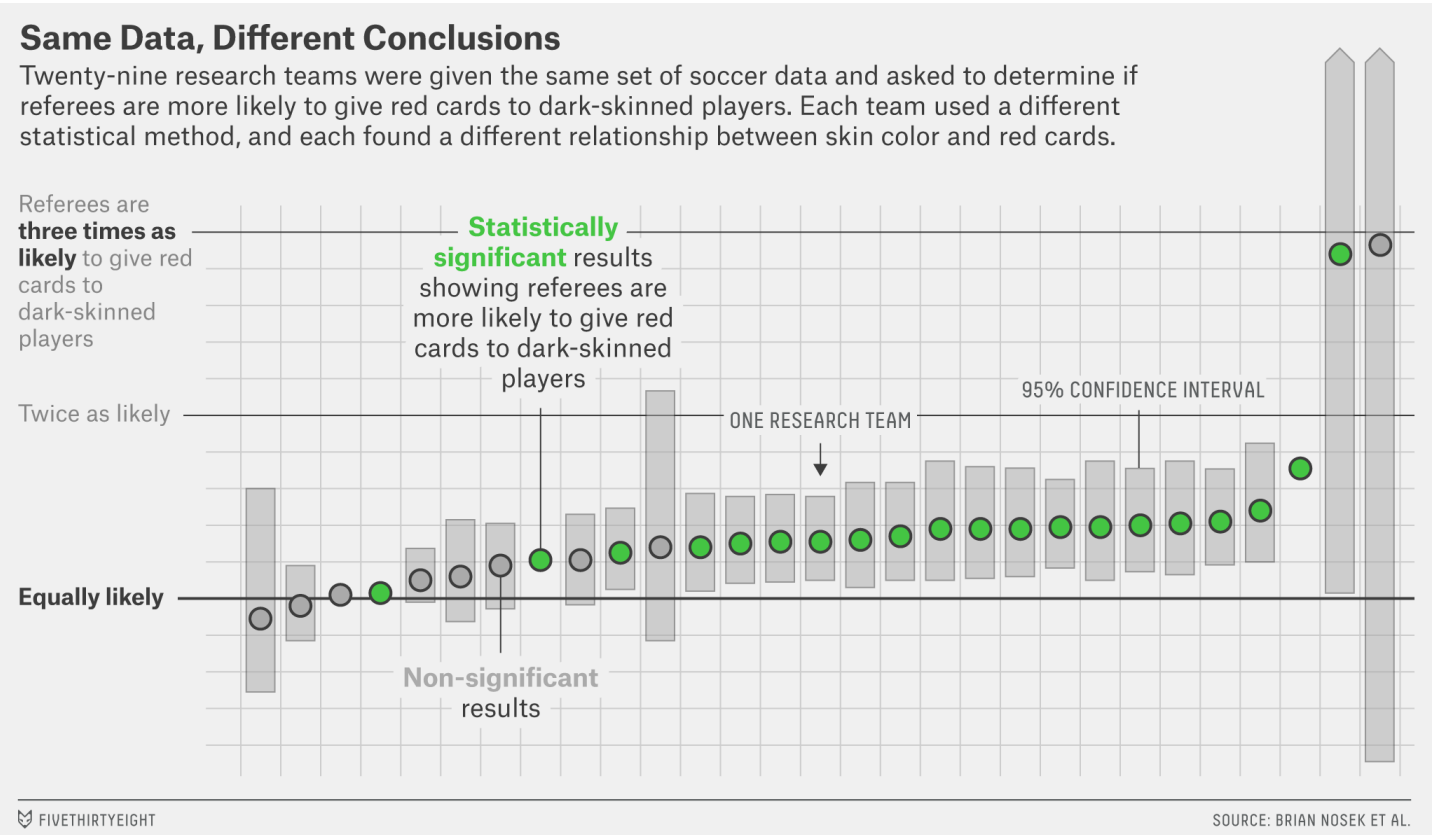
\includegraphics[width=\linewidth]{samedata.png}
\end{figure}
来源：图片来自\url{fivethirtyeight.com}，研究资料来自\url{https://osf.io/j5v8f/}.
\end{frame}

\begin{frame}{元分析的基本步骤}
使用一个PAP或者规范(protocol)来：
\begin{enumerate}
    \item 决定包括哪些研究（作为数据点）
    \item 决定测量那些结果(outcomes)
    \begin{itemize}
        \item 离散(discrete)变量
        \item 连续(continuous)变量
    \end{itemize}
    \item 选择元回归(meta-regression)的模型
    \begin{itemize}
        \item RE 随机影响
        \item FE 固定影响
    \end{itemize}
\end{enumerate}
\end{frame}

\begin{frame}{元分析：腐败信息的影响 (\cite{Incerti2020})}
\begin{figure}
    \centering
    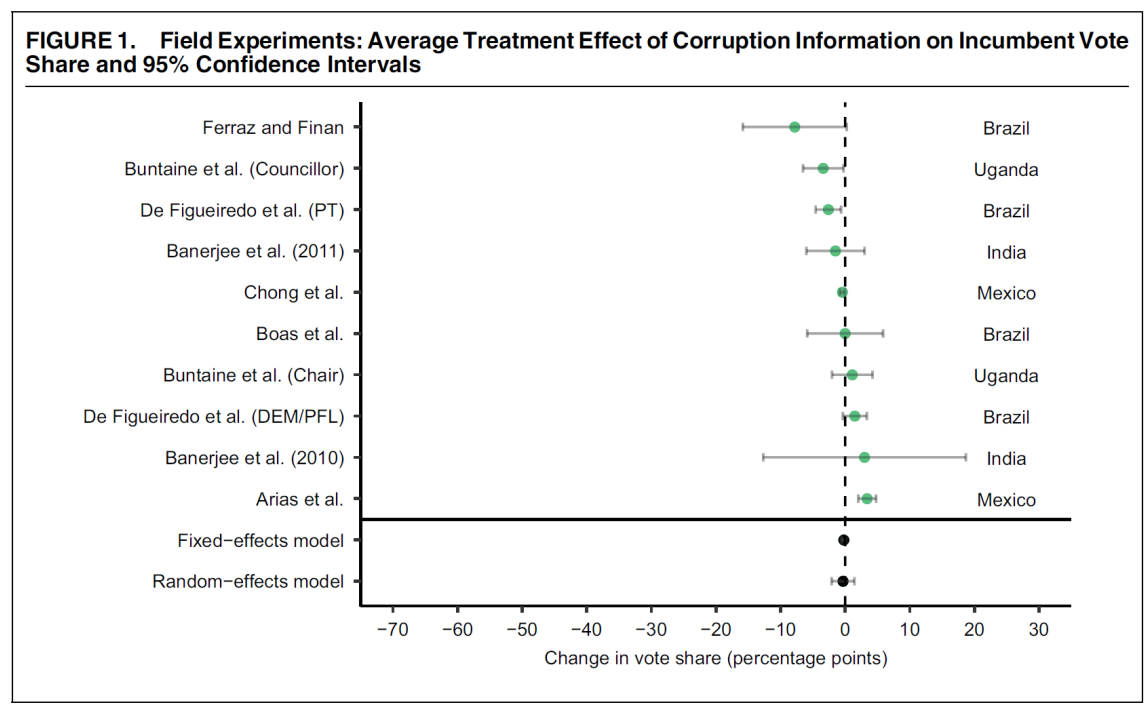
\includegraphics[width=0.9\linewidth]{corruption.png}
\end{figure}
\end{frame}

\begin{frame}{机构(institutional)和学科(discipline)级别的解决方案}
\begin{itemize}
    \item \textbf{基于研究设计的发表：}将数据分析之前的"Registered reports"送审同行评议(peer review)
    \item \textbf{对于透明度(transparency),复现(replication)及元分析(meta-analysis)的激励}
    \begin{itemize}
        \item 详见BITSS  prizes and awards, OSF pre-registration challenge, etc.
    \end{itemize}
    \item \textbf{改变习惯和常态(norms)：}比如说对于数据共享的期刊/学科标准
    \item \textbf{培训(Training)和教育:}BITSS, Center for Open Science, etc.
    \item \textbf{教职：}"Adherence to the replication standard should be part of [tenure] judgment" (\cite{King95})
\end{itemize}
\end{frame}
%---------------------------------------------------------
%Changing visivility of the text

%---------------------------------------------------------
\begin{frame}[allowframebreaks]
\frametitle{References}
\printbibliography
\end{frame}

\end{document}
